\documentclass[UTF8]{ctexbeamer}
%\usepackage[utf8]{inputenc}
\usepackage{pgfpages}
\usepackage{tikz}
\usepackage{animate} % for insert gif
\usepackage{media9}% for insert movie
%\usepackage[UTF8]{ctex}
\usepackage{color}
\usepackage{epsfig}
\usepackage{graphicx}
\usepackage{amsmath}
\usepackage{amssymb}
\usepackage{url}
\usepackage{tikz}
\usepackage{thuthesis}
\usepackage{ IEEEtrantools }
\usepackage{booktabs}
\usepackage{pifont}%for cmark and xmark
%\usefonttheme{default}
%\usetheme{Madrid}
\usetheme{Warsaw}
%\setbeamercovered{transparent}
\setbeamertemplate{footline}[frame number]
\beamertemplatenavigationsymbolsempty  
\usetikzlibrary{arrows,shapes}
\newcommand{\cmark}{\ding{51}}%
\newcommand{\xmark}{\ding{55}}%
%Information to be included in the title page:
\title[Vitiligo Segmentation] %optional
{基于皮肤病图像的白癜风分割}
\subtitle{弱监督方法及``AI落地"}
 
\author[边张行 08015409] % (optional, for multiple authors)
{报告人:边张行(08015409) \and \\~\\指导教师:夏思宇}
 
\institute[SEU] % (optional)
{
\normalsize 东南大学自动化学院, 南京
}
 
\date[June 4, 2019] % (optional)
{2019年6月4日 }
 
\logo{
\includegraphics[height=1cm]{SoutheastUniversity.jpg}}
%\logo{\includegraphics[height=1.5cm]{Automation.jpg}}

\AtBeginSection[] % to put the table of contents at the beginning of each section and highlight the title of the current section.
{
  \begin{frame}
    \frametitle{目录}
    \tableofcontents[currentsection]
  \end{frame}
}
%\setbeamertemplate{navigation symbols}{}

\begin{document}
 
\frame{\titlepage}
 \begin{frame}
\frametitle{目录}
\tableofcontents
\end{frame}

%%%%%%%%  slides  %%%%%%
\section{背景及意义}
\subsection{背景}

\begin{frame}{背景}
\begin{columns}[c]
\column{.55\textwidth}
\begin{enumerate}
\item 影响人数:全球0.5\%--1\%
\item 影响美观
\item 病情评价:面积与脱色程度
\begin{itemize}
\item 方法不客观:医生估算面积
\item 操作不方便:方格纸拓写
\item 标准不统一:VETF\footnote[frame]{\tiny A. Taieb et al. The definition
and assessment of vitiligo: a consensus report of the vitiligo
european task force. Pigment Cell Research, 20(1):27–
35, 2007.},VASI\footnote[frame]{\tiny I. Hamzavi et al. Parametric modeling of narrowband uv-b phototherapy
for vitiligo using a novel quantitative tool: the vitiligo
area scoring index. Archives of Dermatology, 140(6):677–
683, 2004.},SAVASI\footnote[frame]{\tiny L. Komen et al. The validity, reliability and acceptability
of the savasi; a new self-assessment score in vitiligo. Journal
of the European Academy of Dermatology and Venereology,
29(11):2145–2151, 2015.}
\end{itemize}
\end{enumerate}

\column{.5\textwidth}
\begin{figure}
    \centering
    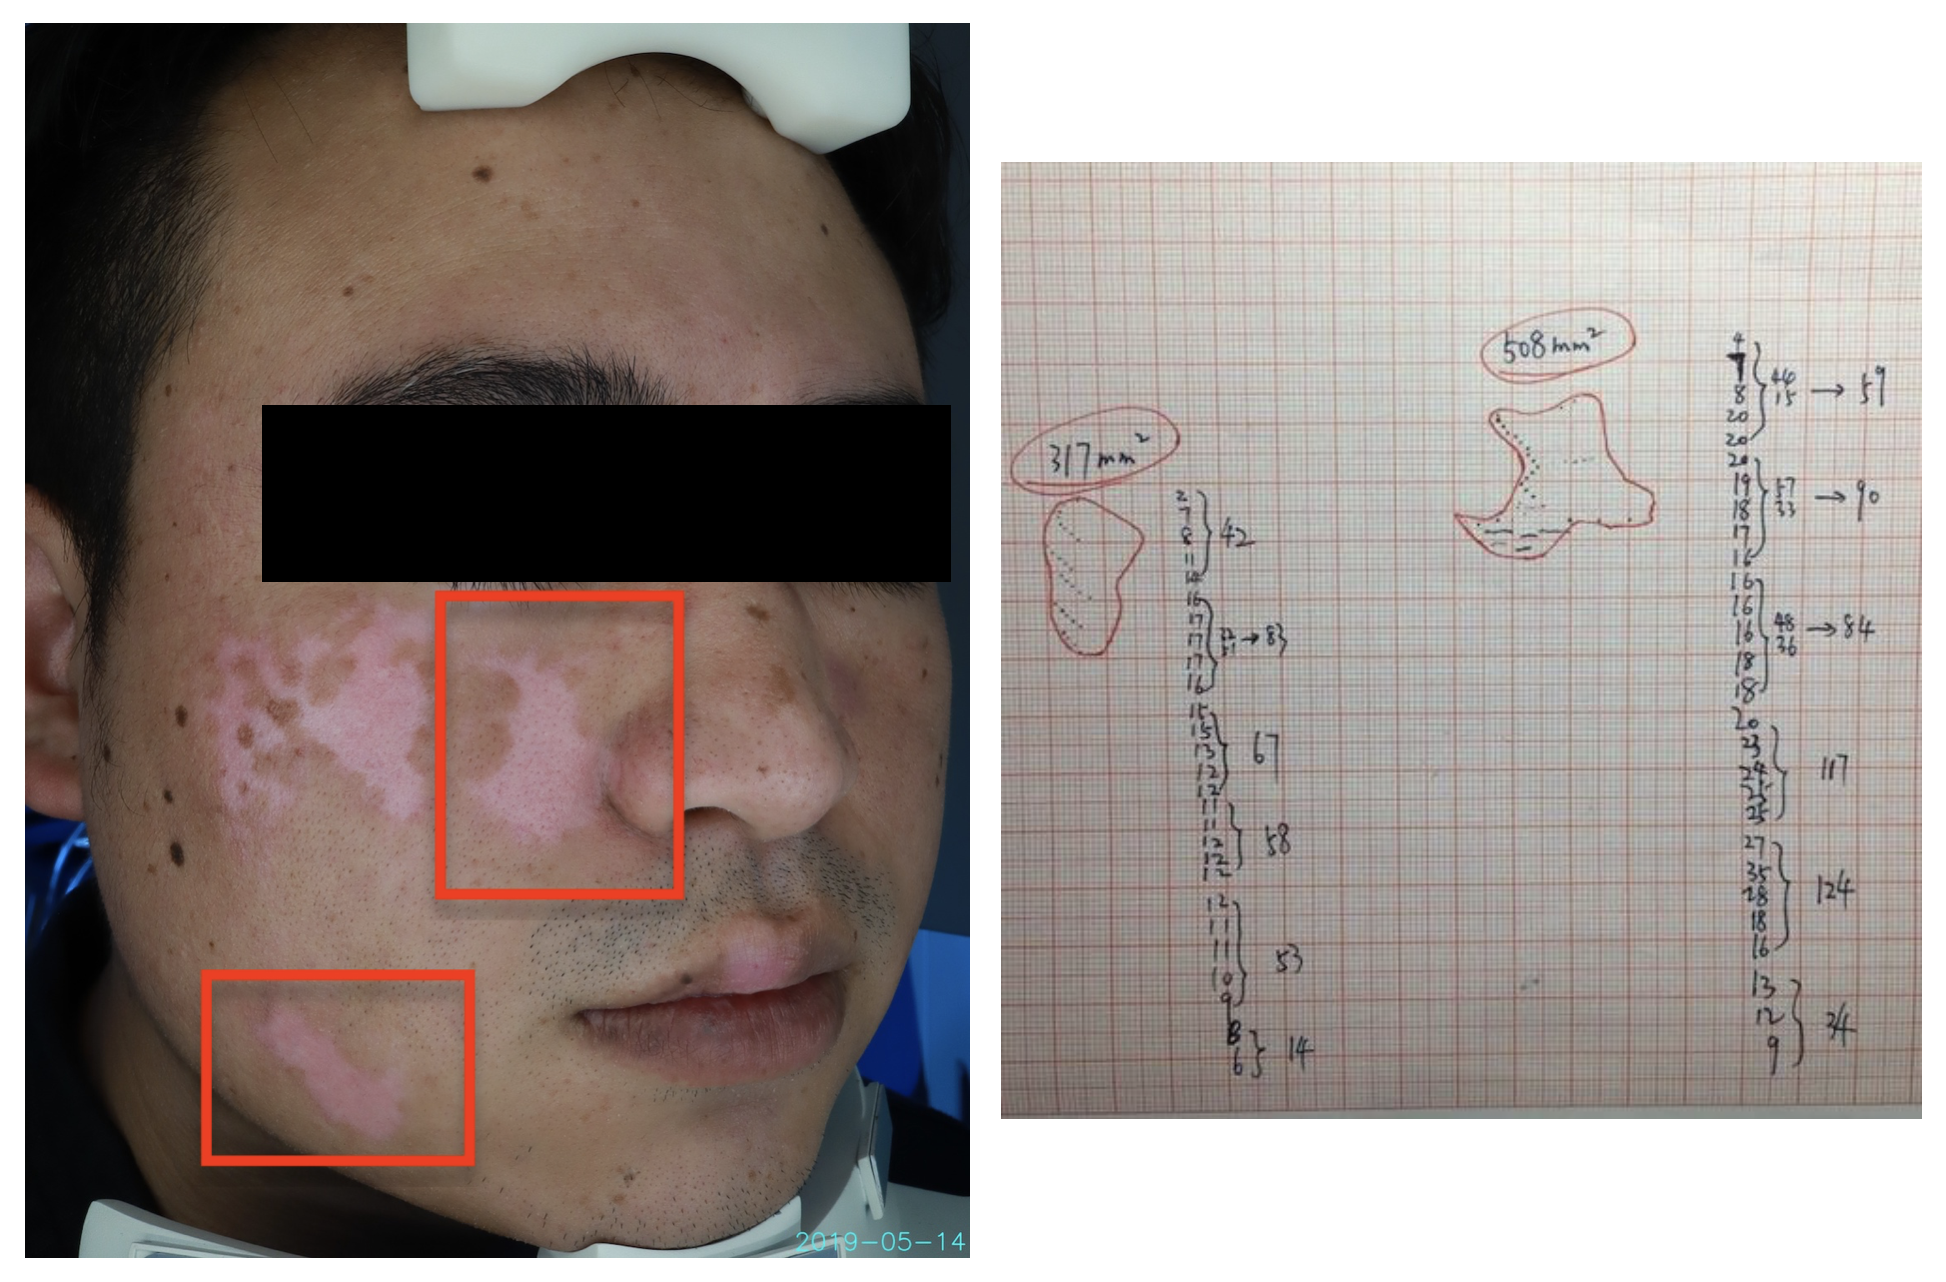
\includegraphics[width=\linewidth]{figures/intro.png}
    \caption{手工拓写}
\end{figure}
\end{columns}
\end{frame}

\subsection{意义}
\begin{frame}{意义}
\begin{itemize}
\item 方法更客观~$\Rightarrow$~数字图像处理:分割任务
\item 操作更方便 (e.g. 远程诊断,随时监控)
\item 标准更统一 
\end{itemize}
\end{frame}






\section{方法原理}
\subsection{强监督分割方法}
%%%
\begin{frame}{强监督分割方法}
\begin{center}
``写在前面:{\color{red}非原创工作均有标注引用}''
\end{center}
\begin{columns}[c]
\column{.6\textwidth}
\begin{figure}
    \centering
    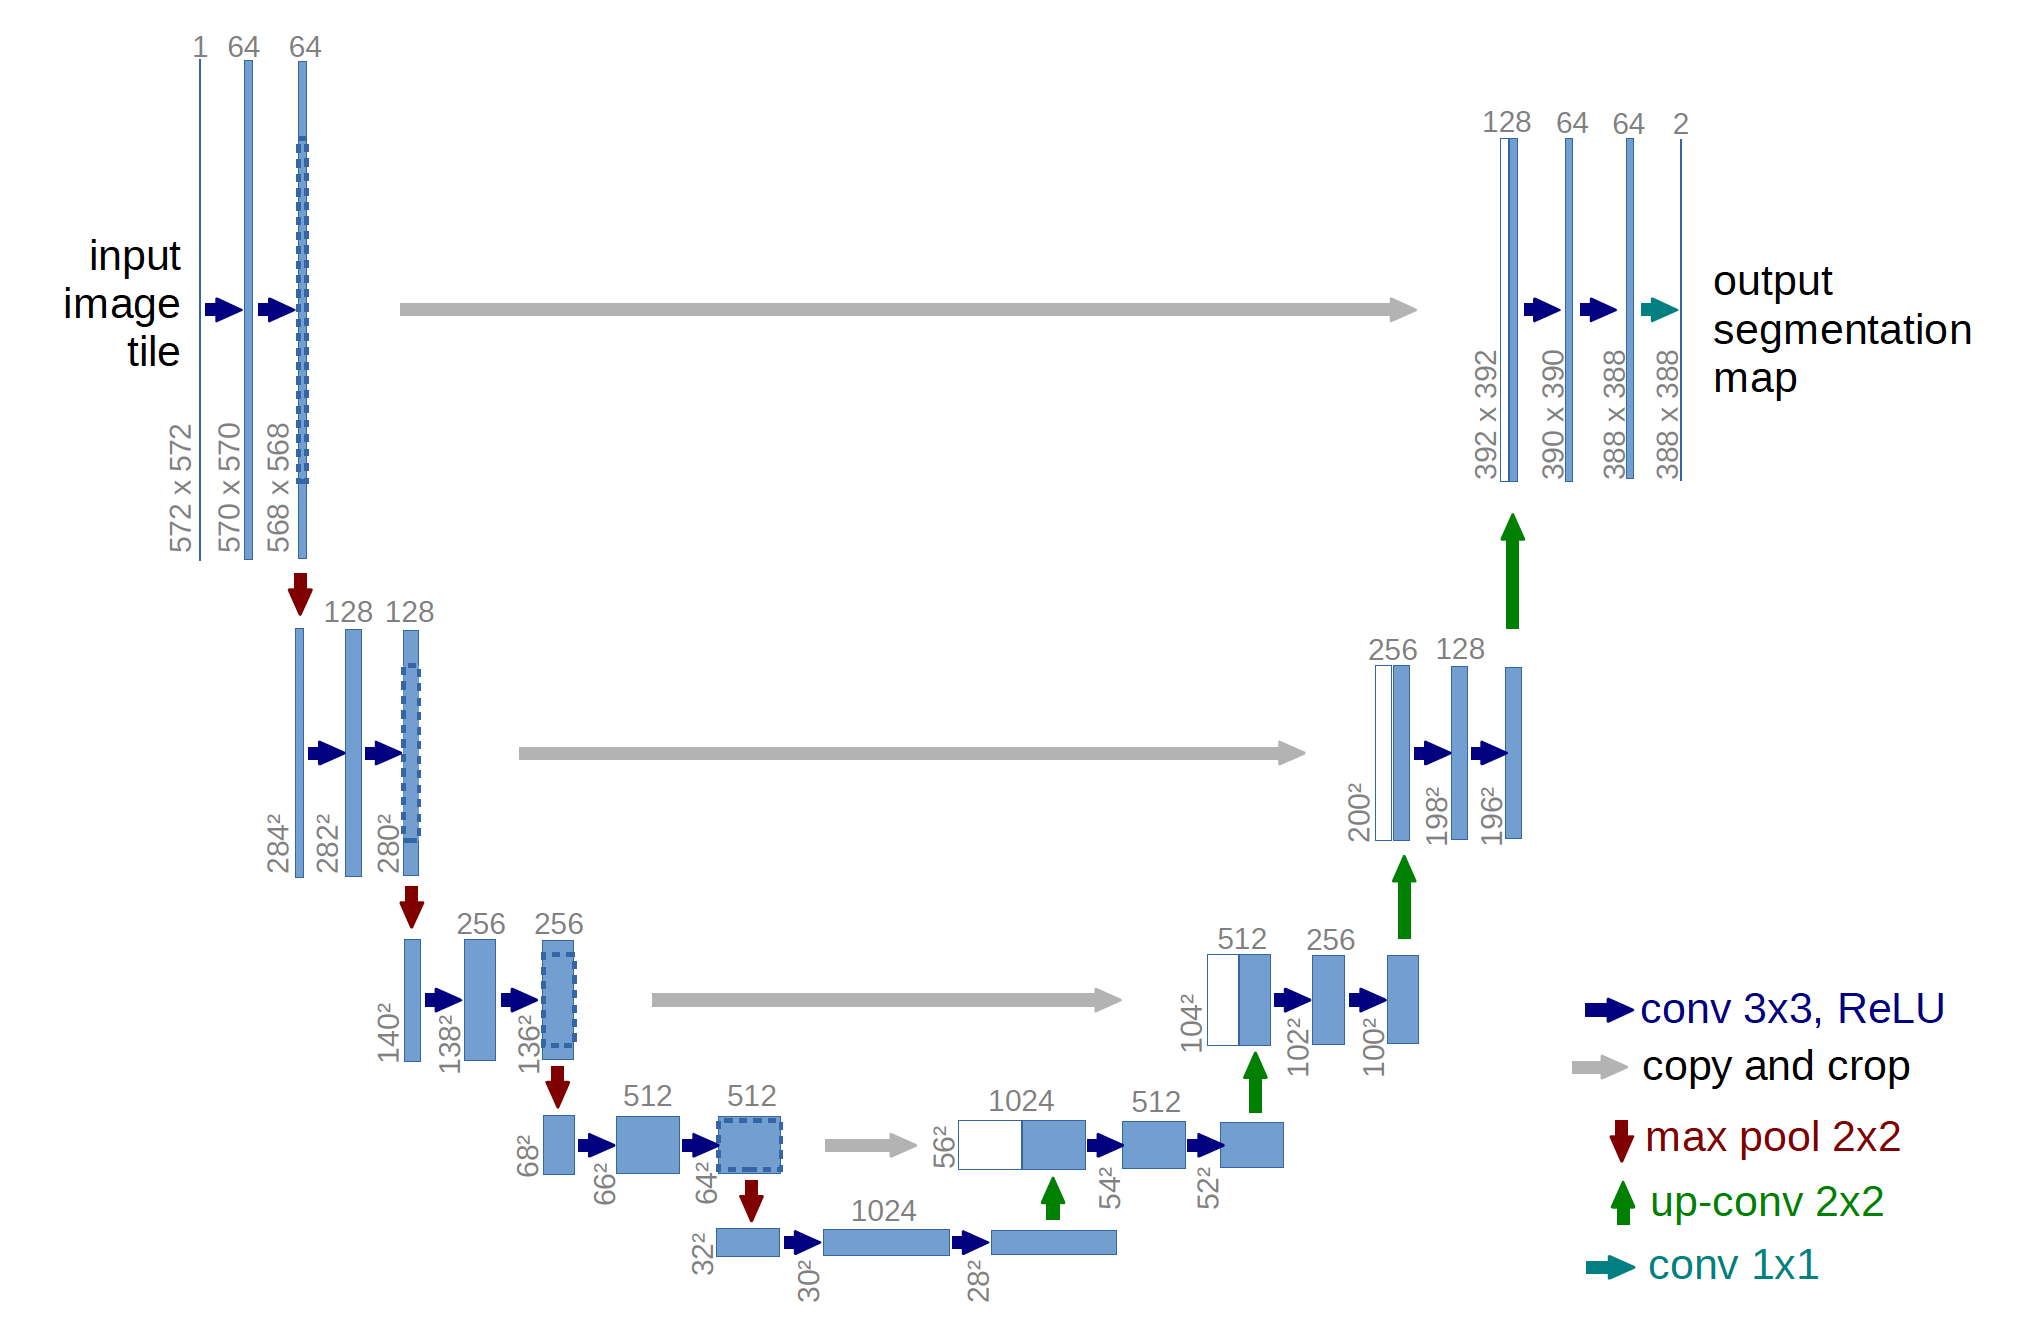
\includegraphics[width=\linewidth]{figures/chap2_Unet.png}
    \caption{编码器-解码器结构\footnote[frame]{\tiny O. Ronneberger, et al. U-net: Convolutional networks for biomedical image segmentation. In International Conference on Medical image computing and computer-assisted intervention, pages 234–241. Springer, 2015.}}
\end{figure}

\column{.5\textwidth}
\begin{itemize}
\item 监督方式:强监督 \pause
\item ``人工智能,有多少智能,就有多少人工''
\item $\Rightarrow$~Vit2019数据集
\end{itemize}
\end{columns}
\end{frame}
%%%
\begin{frame}{数据集Vit2019}
\begin{columns}[c]
\column{.6\textwidth}
\begin{figure}
    \centering
    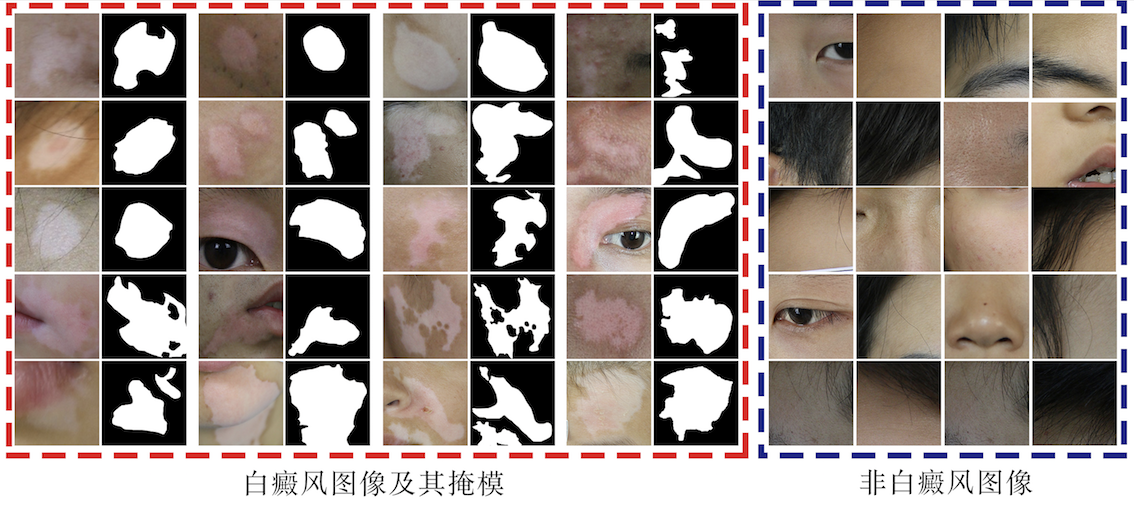
\includegraphics[width=\linewidth]{figures/chap2_DatasetGragh1.png}
    \caption{Vit2019数据集}
\end{figure}

\column{.5\textwidth}
\begin{itemize}
\item 规模:1000+1000
\item 标注:像素级标注
\item 多样性:光照、肤色、不同治疗阶段等
\end{itemize}
\end{columns}

\end{frame}
%%%
\begin{frame}{数据集Vit2019的挑战}
\begin{columns}[c]
\column{.5\textwidth}
\begin{figure}
    \centering
    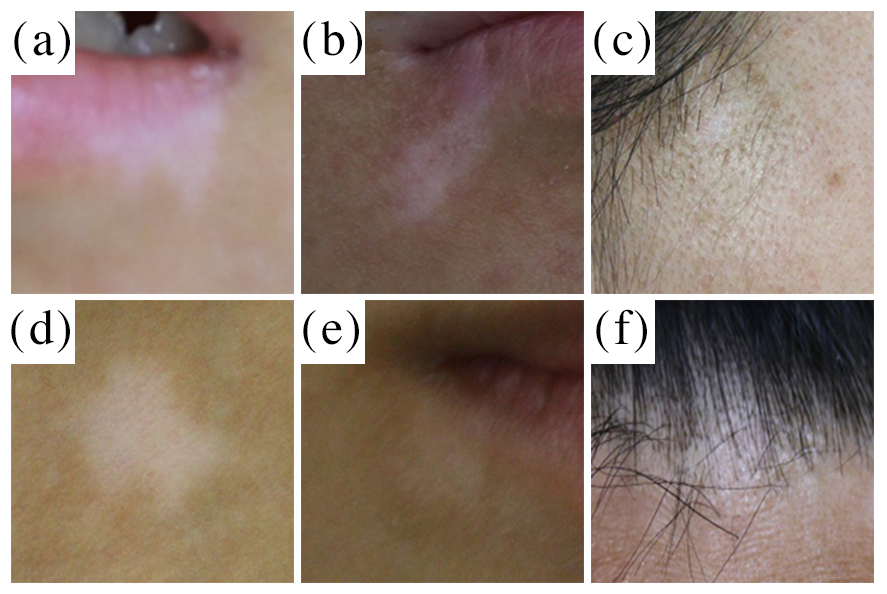
\includegraphics[width=\linewidth]{figures/chap1_challenge.jpg}
\end{figure}

\column{.5\textwidth}
\begin{itemize}
\item 肤色差别大((a) vs. (b))
\item 对比度低((a) , (e))
\item 毛发影响((c) , (f))
\item 局部高光(易误判)((c))
\end{itemize}
\end{columns}
\end{frame}
%%%
\begin{frame}{Baseline: Unet\footnote[frame]{\tiny O. Ronneberger, et al. U-net: Convolutional networks for biomedical image segmentation. In
International Conference on Medical image computing and computer-assisted intervention, pages 234–241. Springer, 2015.}}
\begin{columns}[c]
\column{.5\textwidth}
\begin{figure}
    \centering
    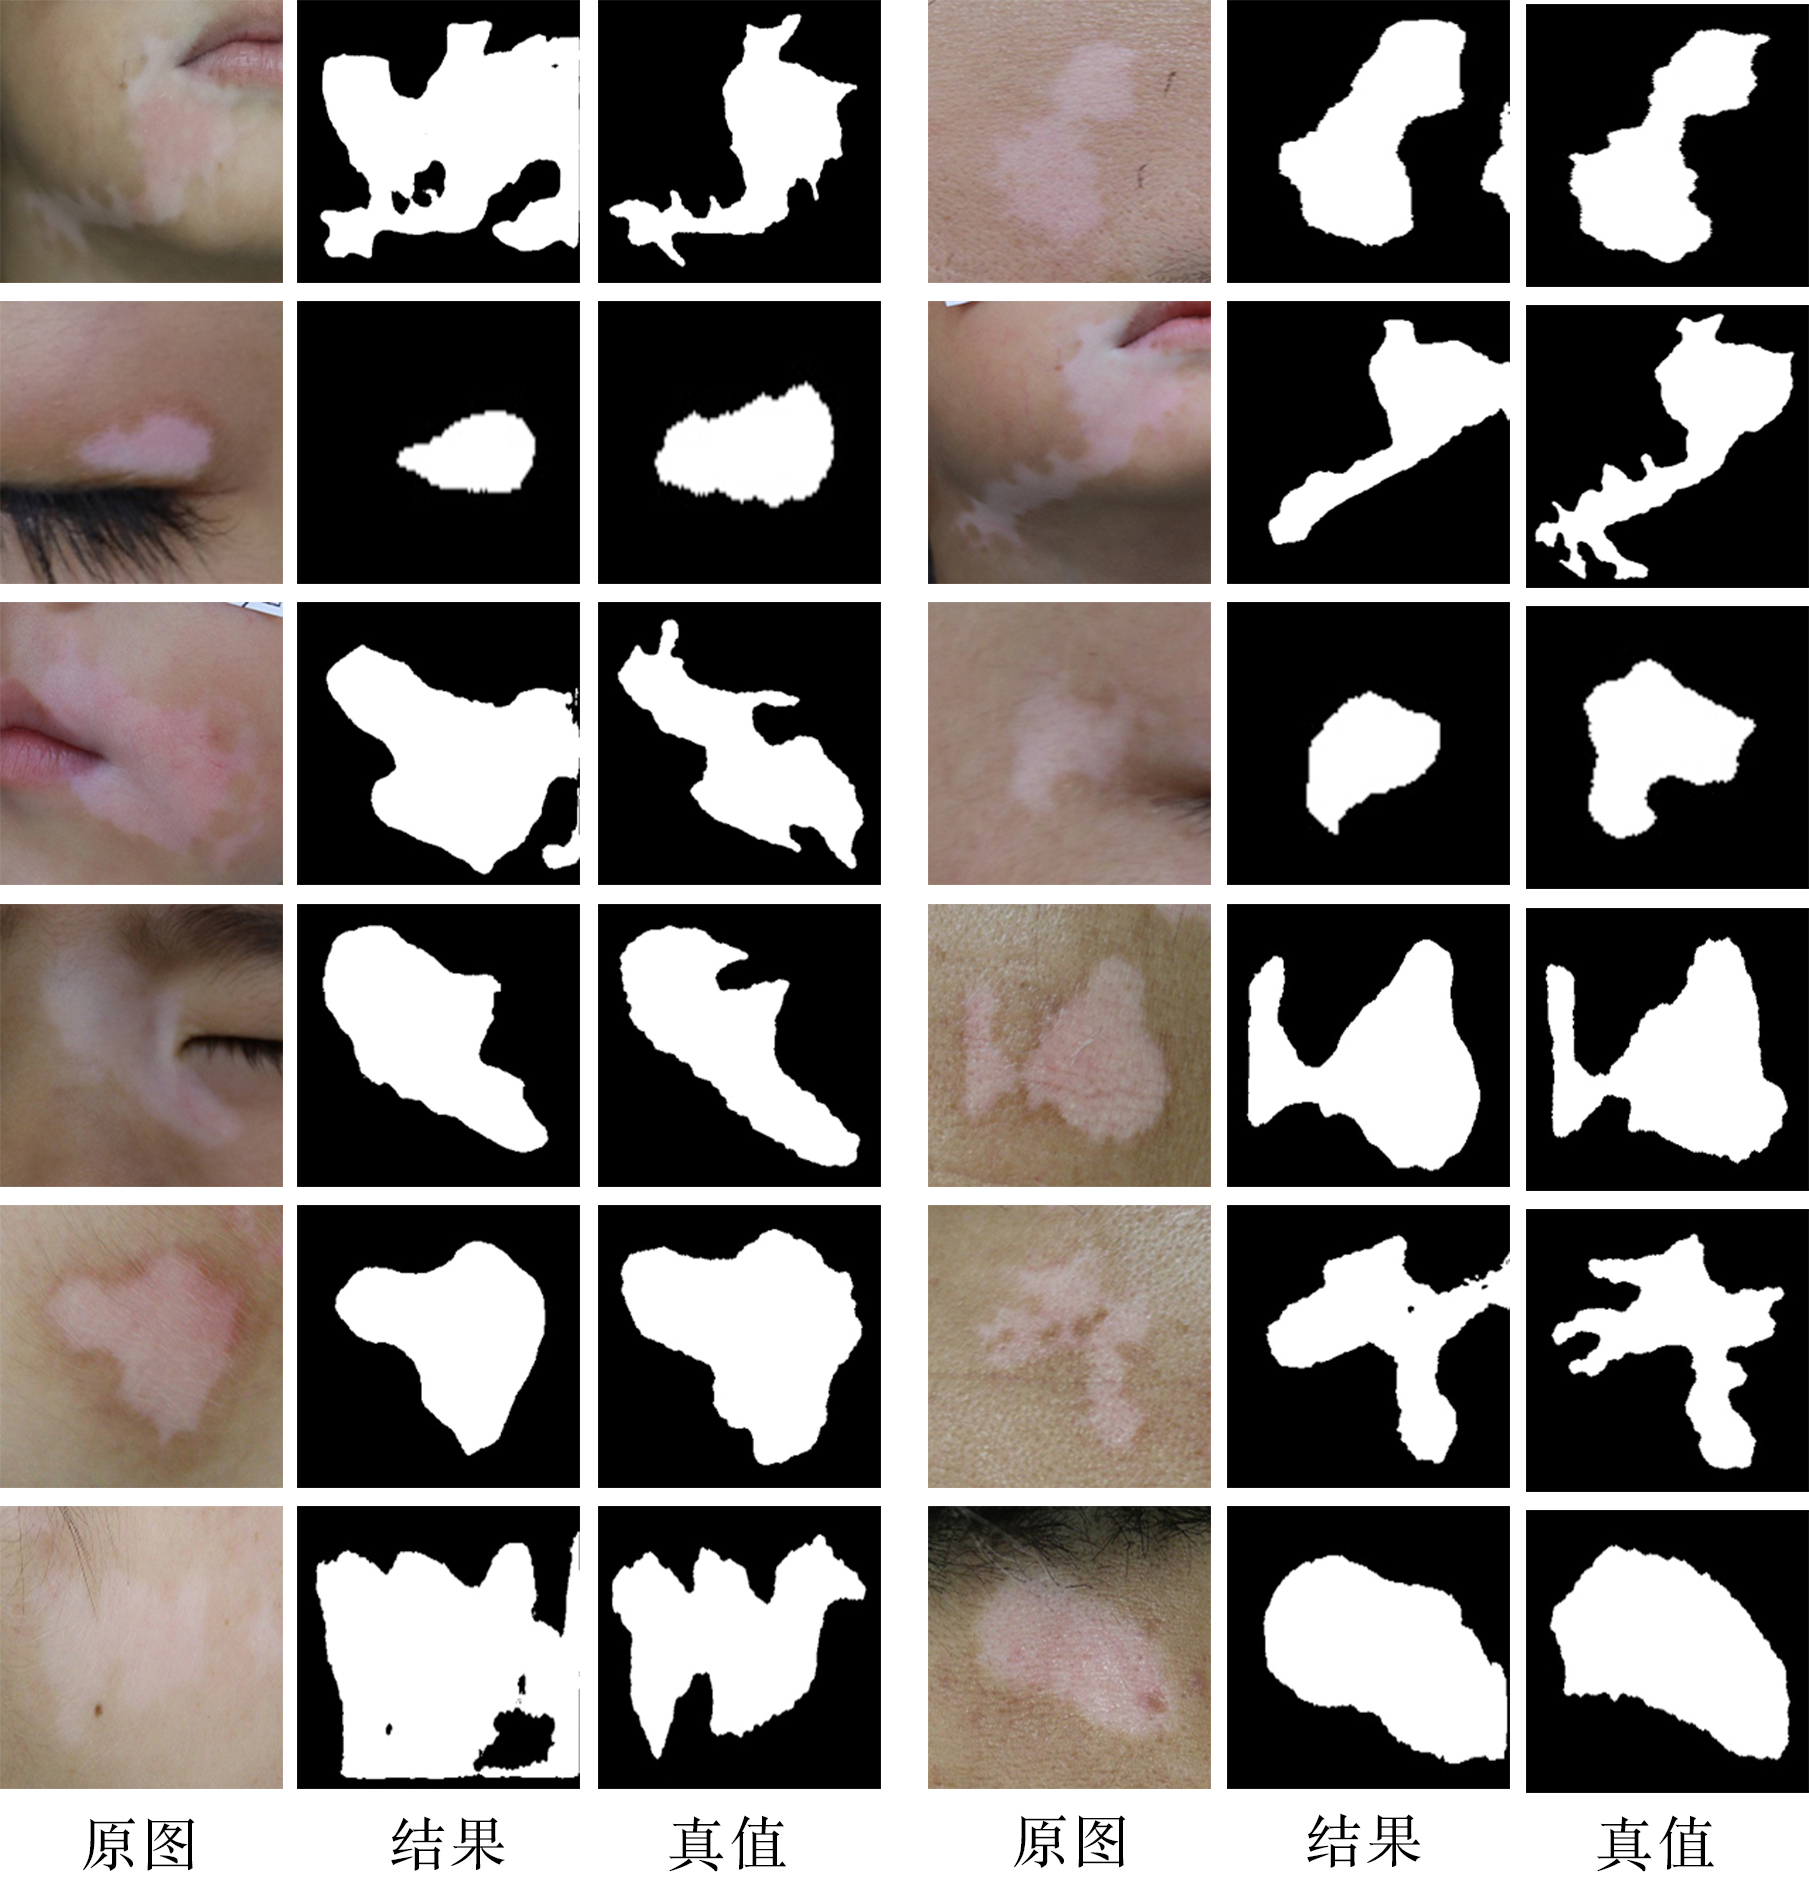
\includegraphics[width=\linewidth]{figures/UnetResult.jpg}
\end{figure}

\column{.45\textwidth}

\begin{IEEEeqnarray}{rCl}
\label{eq:1}
\mathrm{IoU}=&&\frac{\mathrm {Area\,of\,Overlap}}{\mathrm {Area\,of\,Union}} \nonumber \\
\nonumber \\ 
=&&78.6\% \nonumber
\end{IEEEeqnarray}
\begin{itemize}
\item 强监督方法局限性: \\ 数据标注工作耗时耗力
\end{itemize}
\end{columns}
\end{frame}
%%%
\subsection{弱监督分割方法}
\begin{frame}{弱监督分割框架}
\begin{figure}
    \centering
    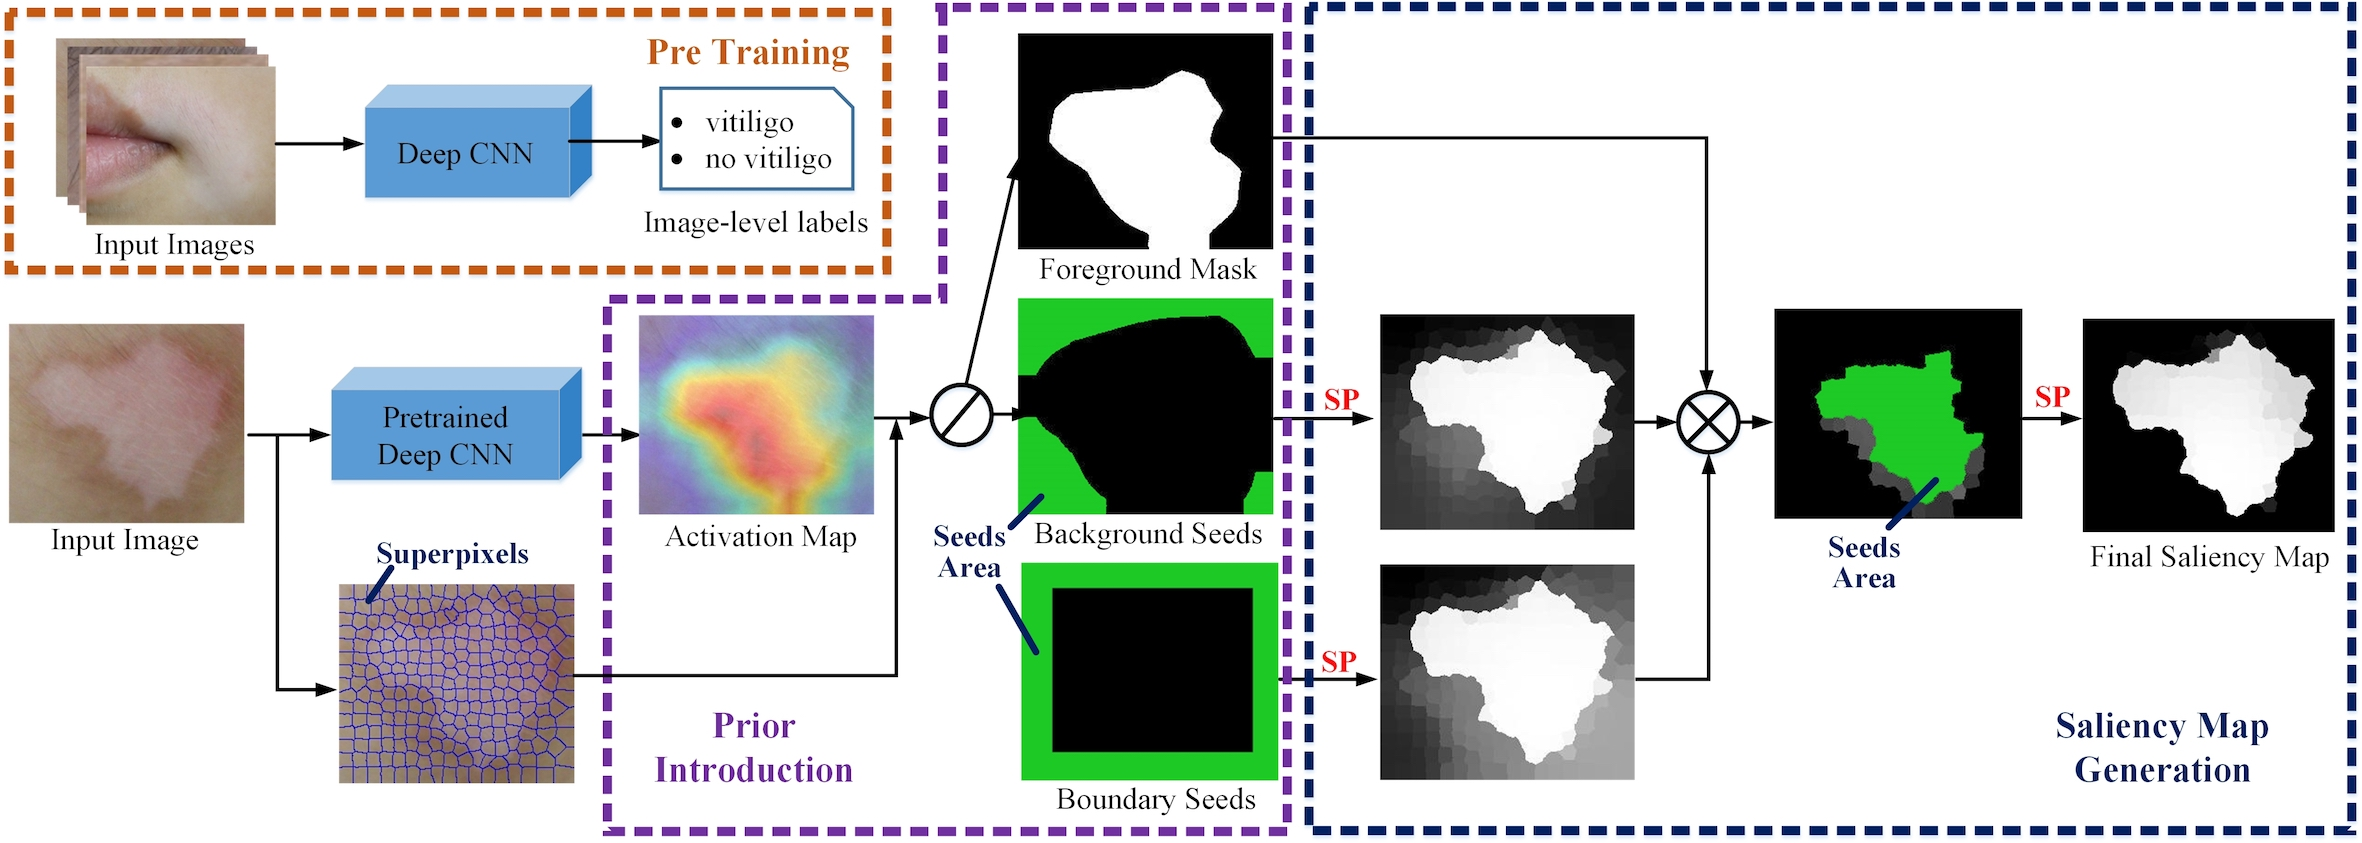
\includegraphics[width=\linewidth]{figures/CNNandSuperPixelModelGraph3.jpg}
\end{figure}
\vfill
\begin{itemize}
\item 超像素分割
\item 高层语义特征+底层特征 ---``既见树木,又见森林''
\item 将反馈应用于显著性传播过程
\end{itemize}
\end{frame}
%%%

\begin{frame}{超像素分割}
\begin{columns}[c]
\column{.6\textwidth}
\begin{figure}
    \centering
    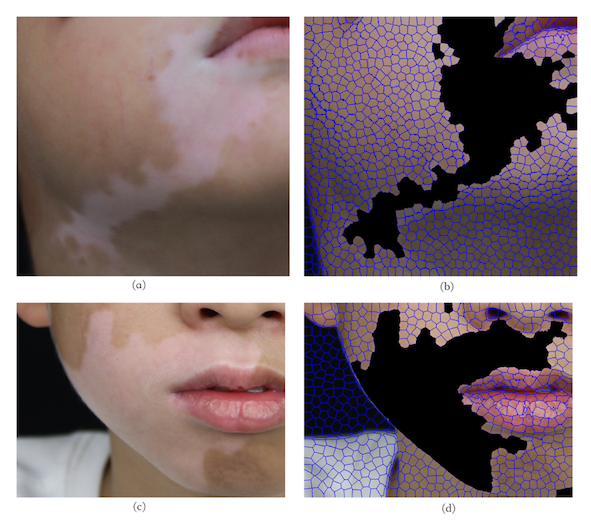
\includegraphics[width=\linewidth]{figures/chap3_SLICresult2.png}
\end{figure}

\column{.45\textwidth}
好处:
\begin{itemize}
\item 降低数据维度
\item 剔除异常像素点
\item 保留较完整的皮损边界
\end{itemize}
\end{columns}
\end{frame}
%%%
\begin{frame}{``既见树木,又见森林''}
\begin{block}{定义}
``森林'': 高层特征 $\Rightarrow$ 定位种子区域

``树木'':底层特征 $\Rightarrow$ 传播
\end{block}

\vfill 
\pause
\begin{itemize}
\item 定位:类激活图\footnote[frame]{\tiny Zhou, Bolei, et al. Learning deep features for discriminative localization. CVPR 2016.} ( {\color{red}C}lass {\color{red}A}ctivation {\color{red}M}ap -- {\color{red}CAM})
\begin{figure}
    \centering
    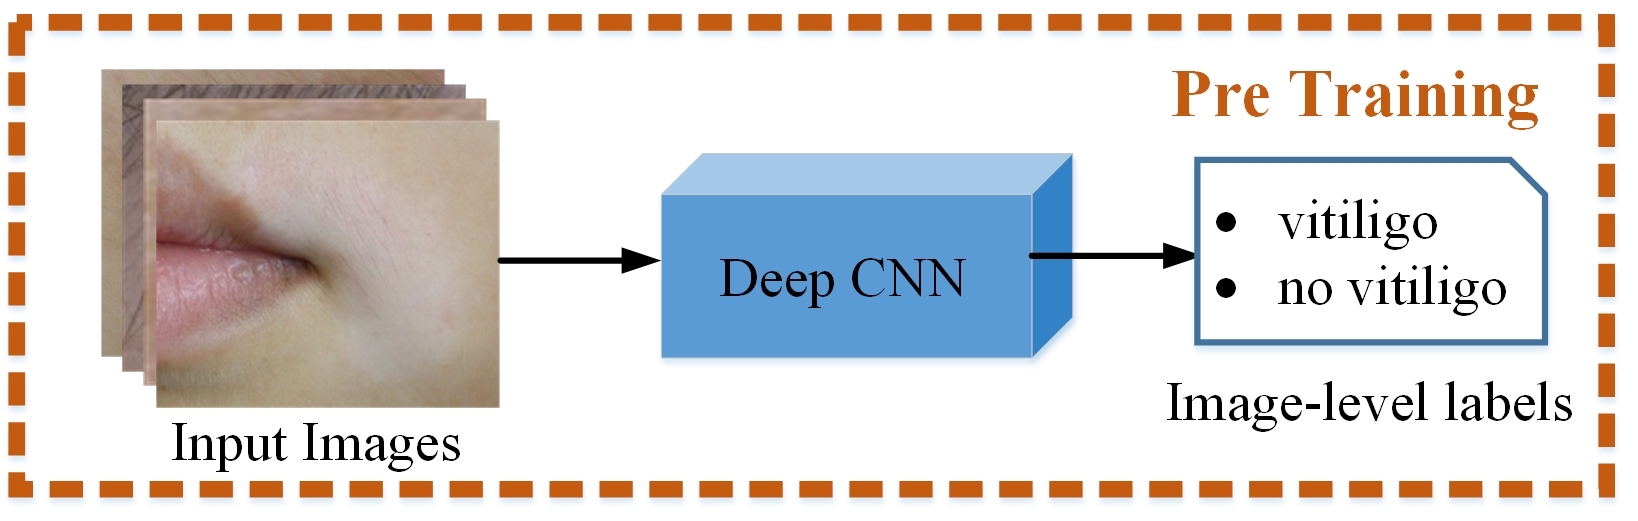
\includegraphics[width=0.5\linewidth]{figures/TrainForCam.jpg}
\end{figure}
\end{itemize}

\vspace{-0.2cm}

\begin{figure}
    \centering
    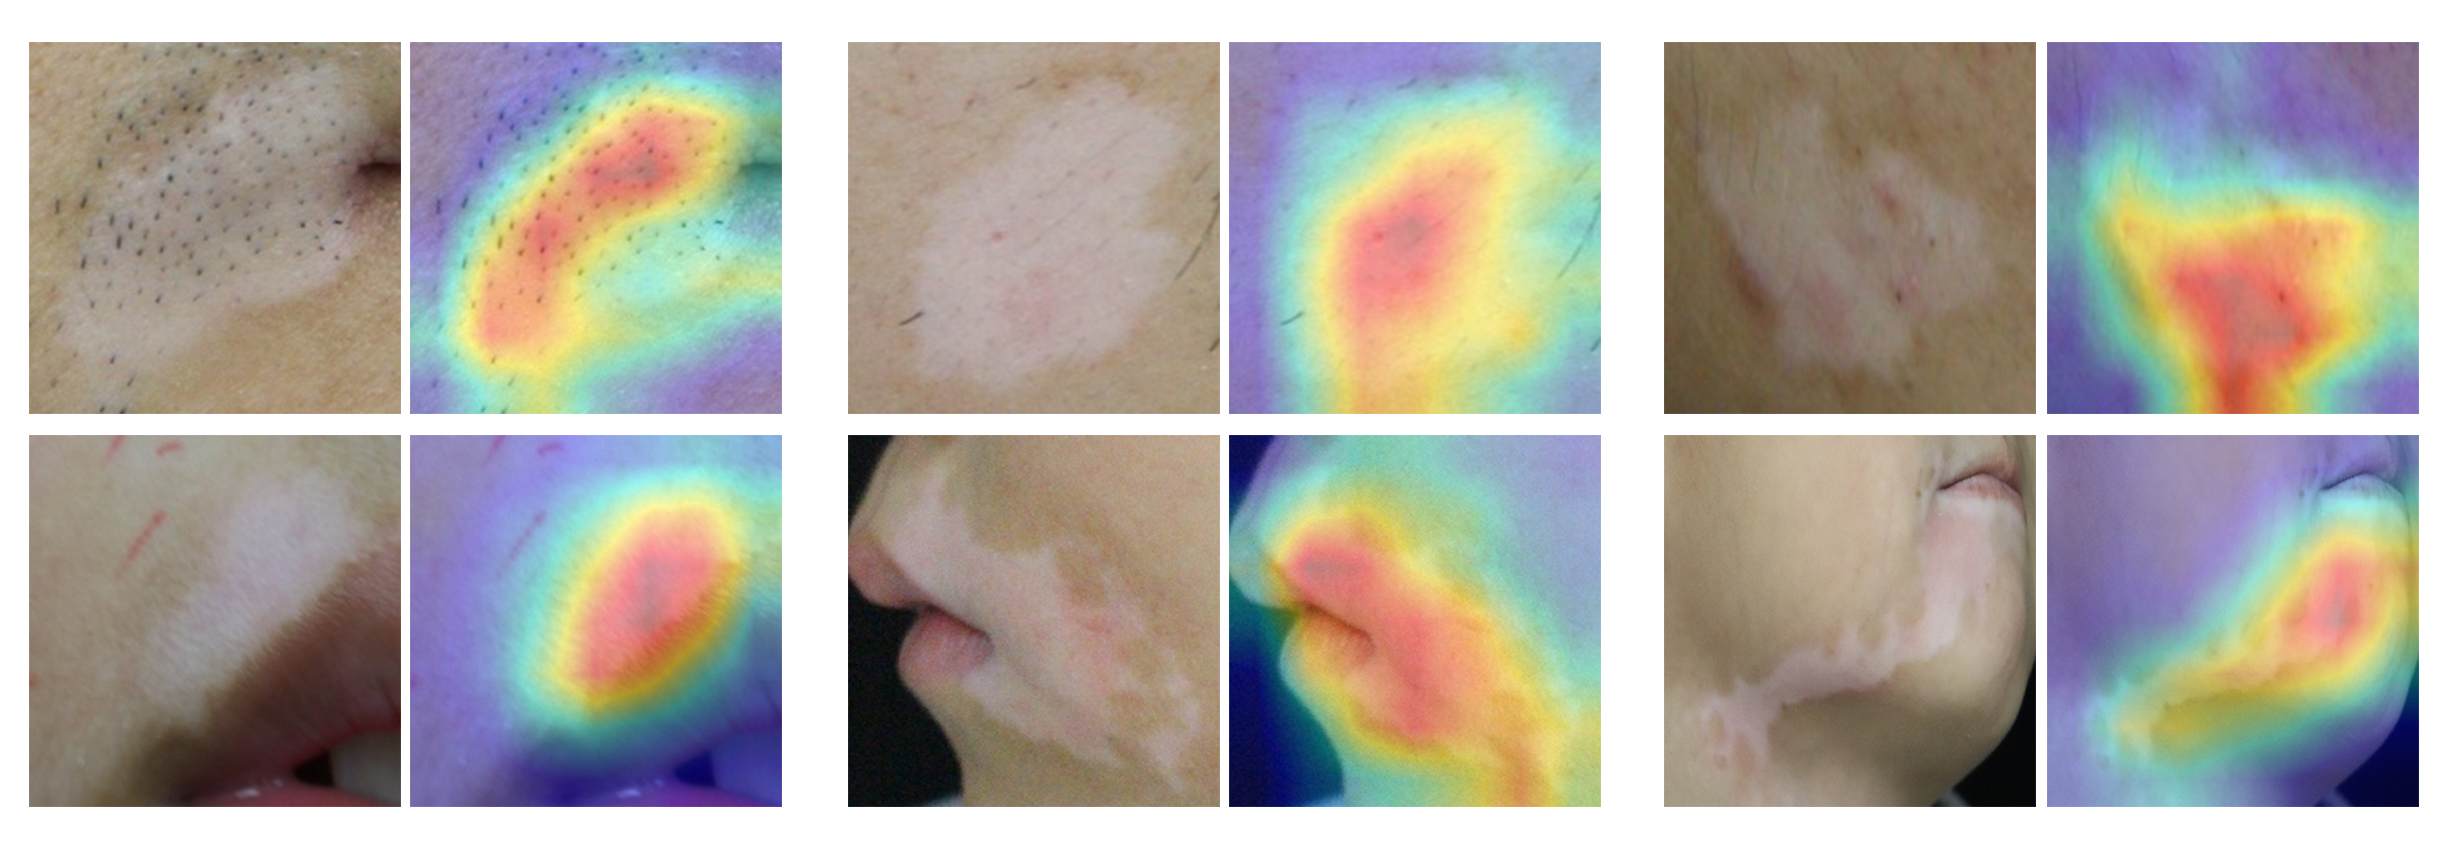
\includegraphics[width=0.65\linewidth]{figures/cam.jpg}
\end{figure}

\end{frame}
%%%
\begin{frame}{``既见树木,又见森林''}
\begin{block}{定义}
``森林'': 高层特征 $\Rightarrow$ 定位种子区域

``树木'':底层特征 $\Rightarrow$ 传播
\end{block}
\vfill
传播:
\begin{columns}[c]
\column{.6\textwidth}
\begin{figure}
    \centering
    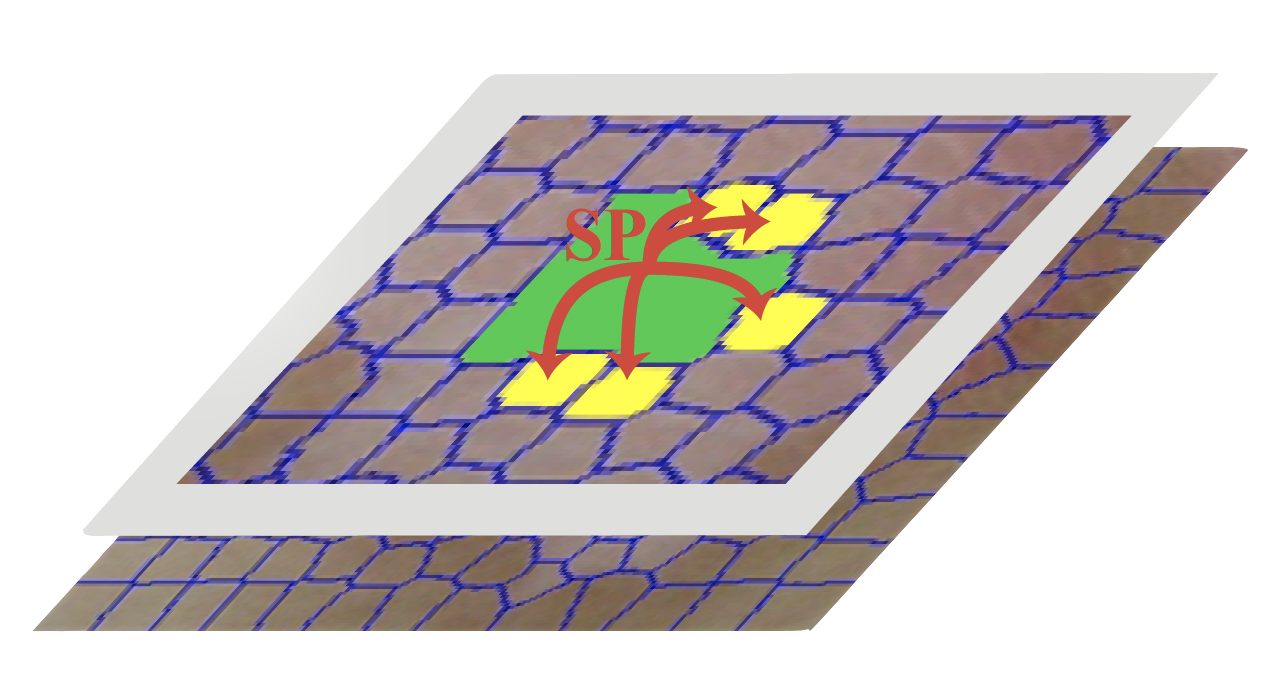
\includegraphics[width=.9\linewidth]{figures/propagationillustrator.png}
\end{figure}

\column{.5\textwidth}
\begin{itemize}
\item 传播过程迭代化
\item 每一次迭代需要确定传播的{\color{blue}{顺序}}\footnote[frame]{\tiny C. Gong et al. Saliency propagation from simple to difficult. CVPR 2015.}和{\color{blue}{数量}}
\end{itemize}
\end{columns}

\end{frame}
%%%
\begin{frame}{``既见树木,又见森林''--传播}

\begin{columns}[c]
\column{.5\textwidth}
\begin{figure}
    \centering
    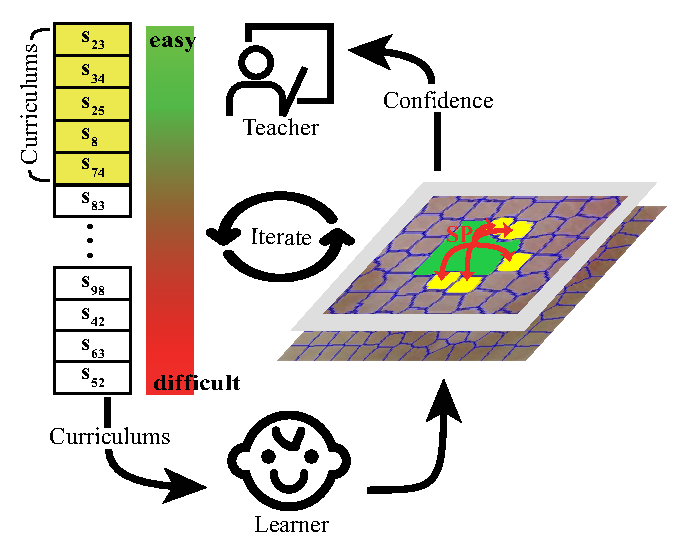
\includegraphics[width=\linewidth]{figures/TLLTillustrator.eps}
    \caption{反馈思想与传播相结合}
\end{figure}

\column{.6\textwidth}
\begin{itemize}
\item 传播过程~$\Rightarrow$~``教学-学习''
\item 老师:
\begin{itemize}
\item 评估课程难度,从易到难布置一定数量的课程;
\item 接受学生反馈
\end{itemize}
\item 学生:
\begin{itemize}
\item 学习课程(传播);
\item 反馈学习效果(confidence)
\end{itemize}
\end{itemize}
\begin{block}{数量}
\small $q^{(t)}={|\mathrm{\#Neighbor^{(t)}}|\times \mathrm{Confidence}^{(t-1)}}$
\end{block}
\end{columns}
\end{frame}
%%%
\begin{frame}{``既见树木,又见森林''--传播}

\begin{block}{老师度量``课程''难度}
$DS_i=INF_i+IND_i+IHM_i+CON_i$
\begin{itemize}
\item 信息性:$INF_i=H(\mathbf{s}_i \mid \mathcal{L})$
\item 个体性:$IND_i=\frac{1}{|\mathcal{N}(\mathbf{s}_i)|}\sum_{j\in \mathcal{N}(\mathbf{s}_i)}\| \mathbf{s}_i^{\mathrm color}-\mathbf{s}_j^{\mathrm color}\|$
\item 同质性:$IHM_i=\Big (\frac{2}{b^2-b}\sum_{i=1}^b \sum_{j=i+1}^b\pmb{\Theta}_{ij}\Big )^{-1}$
\item 连通性:$CON_i=\frac{1}{l}\sum_{j\in \mathcal{L}}\mathrm{geo}({\mathbf{s}_i,\mathbf{s}_j})$
\end{itemize}
\end{block}

\begin{block}{学生反馈效果}
$\mathrm{Confidence}=1-\frac{2}{q^{(t-1)}}\sum_{i=1}^{q^{(t-1)}}\min{(f_i^{(t-1)},1-f_i^{(t-1)})}$
\end{block}
\end{frame}
%%%
\begin{frame}{方法框架}
\begin{figure}
    \centering
    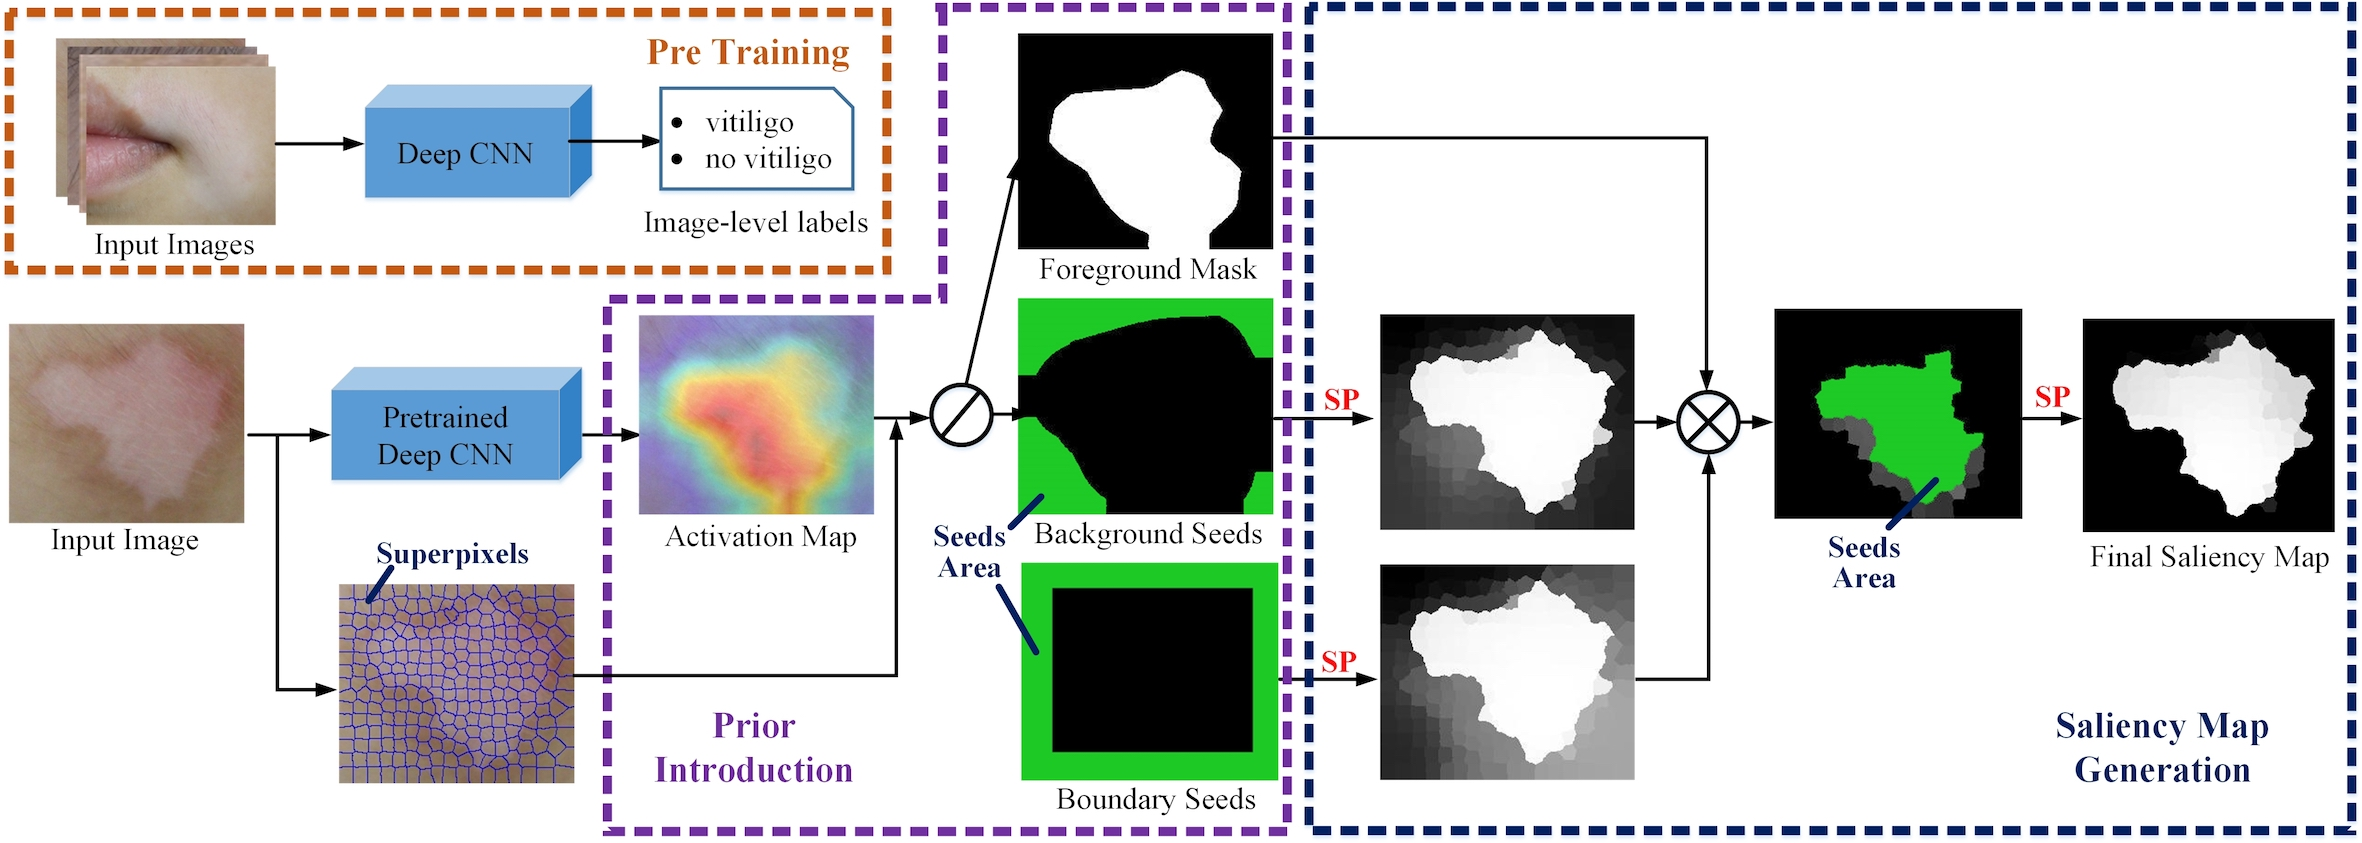
\includegraphics[width=\linewidth]{figures/CNNandSuperPixelModelGraph3.jpg}
\end{figure}
\begin{itemize}
\item 边界先验(Boundary Prior): 假设边界为背景区域
\item 三次显著性传播过程({\color{red}SP})
\end{itemize}
\end{frame}





























\section{实验结果与分析}
\begin{frame}{注意力机制}
\begin{itemize}
\item 注意力机制:Ours vs. TLLT\footnote[frame]{\tiny C. Gong et al. Saliency propagation from simple to difficult. CVPR 2015.}
\begin{figure}
    \centering
    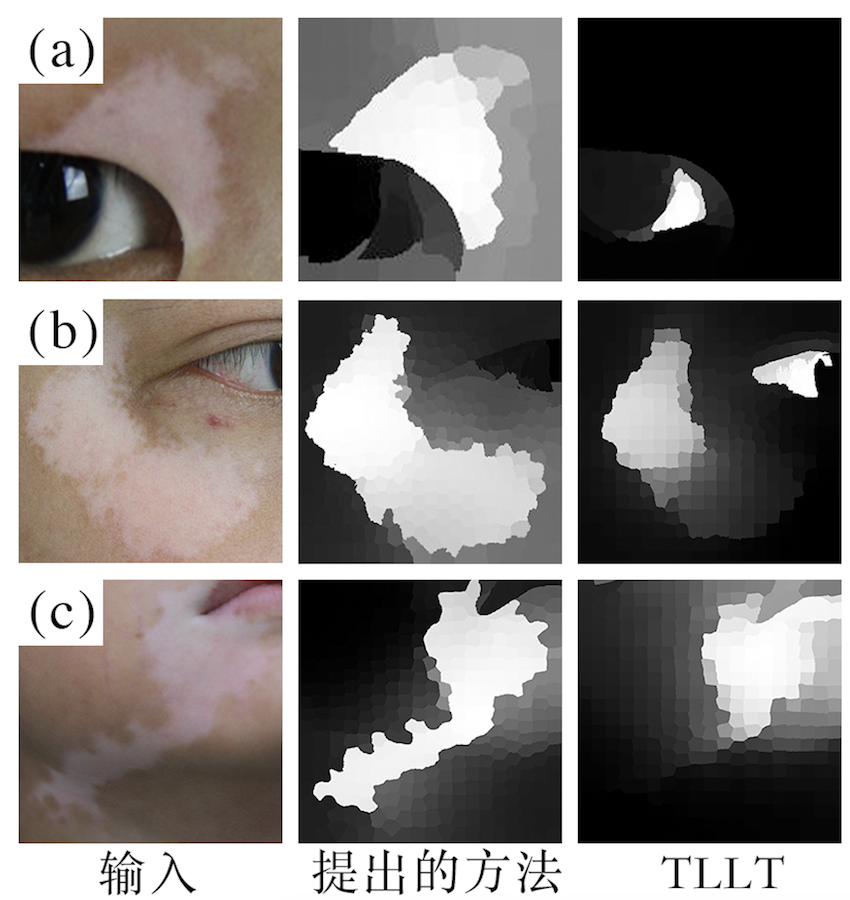
\includegraphics[width=.5\linewidth]{figures/TLLT.png}
\end{figure}
\end{itemize}

\end{frame}

%%%
\begin{frame}{方法对比:Ours vs. Unet}
\begin{columns}[c]
\column{.6\textwidth}
\begin{table}
  \caption{实验结果(Vit2019)}
    \begin{tabular}{c|c|c}
    \toprule
   方法 & 监督方式 & mIoU \\
    \hline
    \hline
    FCN-VGG16  & \multirow{2}[2]{*}{Fully} & 72.4 \\
    U-net &       & 78.6 \\
    \hline
    PRM  & \multirow{3}[2]{*}{Weakly} & 67.2 \\
    SEC  &       & 64.7 \\
    Our Method &       &\textbf{71.4}\\
    \bottomrule
    \end{tabular}%
\end{table}%

\column{.5\textwidth}
\begin{figure}
    \centering
    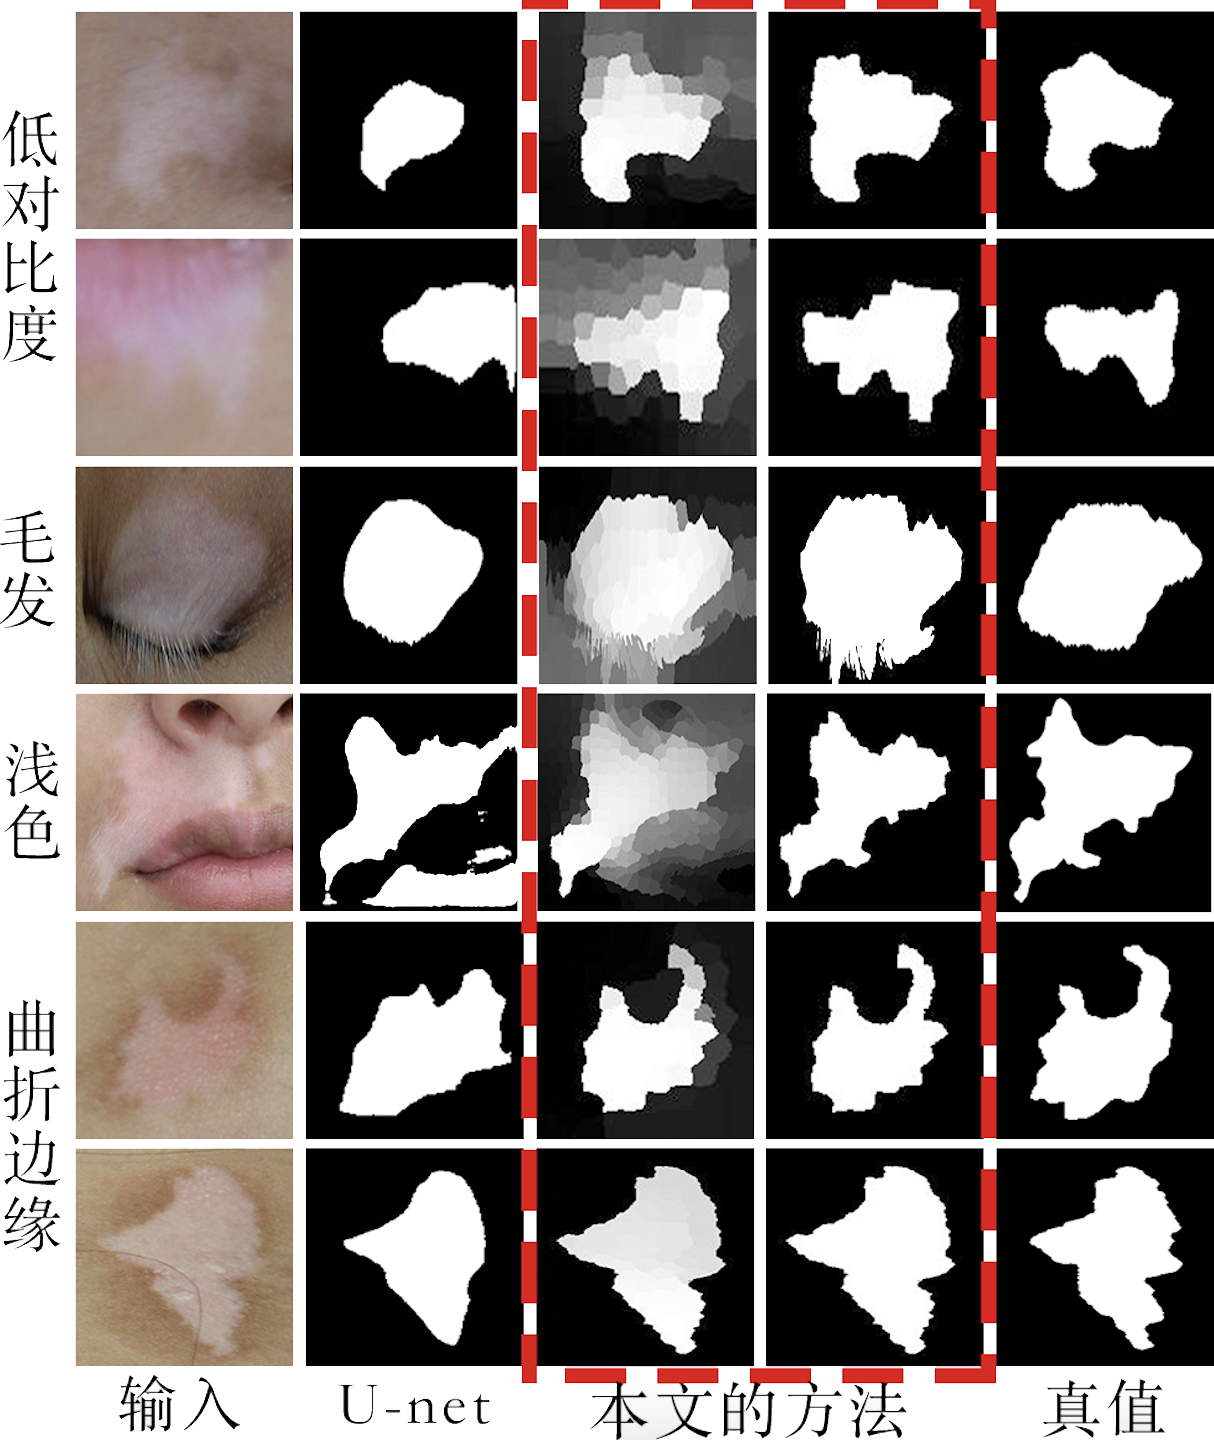
\includegraphics[width=\linewidth]{figures/unetcompareSmaller.png}
\end{figure}
\end{columns}
\end{frame}

%%%
\begin{frame}{方法对比:Ours vs. SEC,PRM}
\begin{figure}
    \centering
    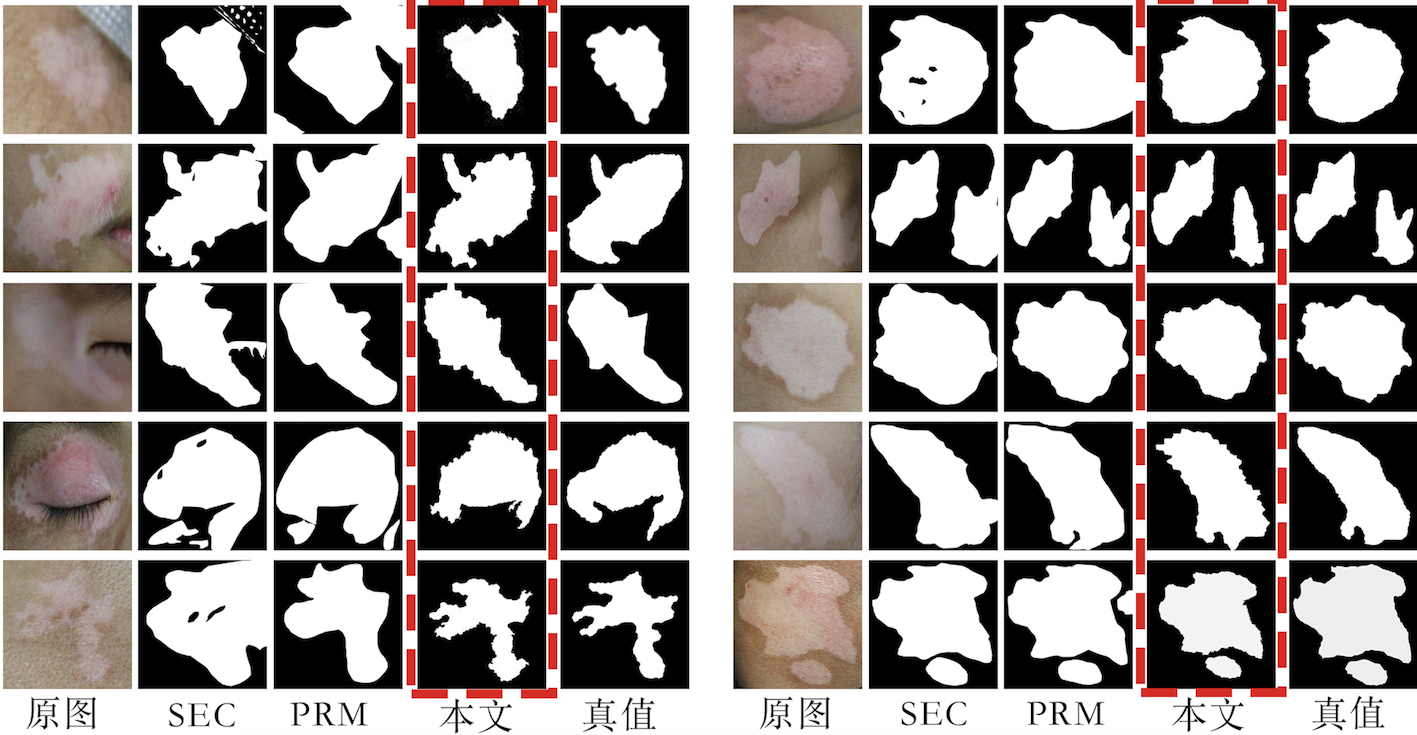
\includegraphics[width=.95\linewidth]{figures/weaklySupervisedCompare.png}
    \vspace{-.5em}
    \caption{弱监督方法效果对比:Ours vs. SEC\footnote[frame]{\tiny A. Kolesnikov and C. H. Lampert. Seed, Expand and Constrain:
Three Principles for Weakly-Supervised Image Segmentation. arXiv.org, Mar. 2016.},PRM\footnote[frame]{\tiny Y. Zhou et al. Weakly Supervised Instance Segmentation using Class Peak Response. arXiv.org, Apr. 2018.}}
\end{figure}
\end{frame}
%%%
\begin{frame}{显著图质量分析}
\begin{columns}[c]
\column{.4\textwidth}
\begin{figure}
    \centering
    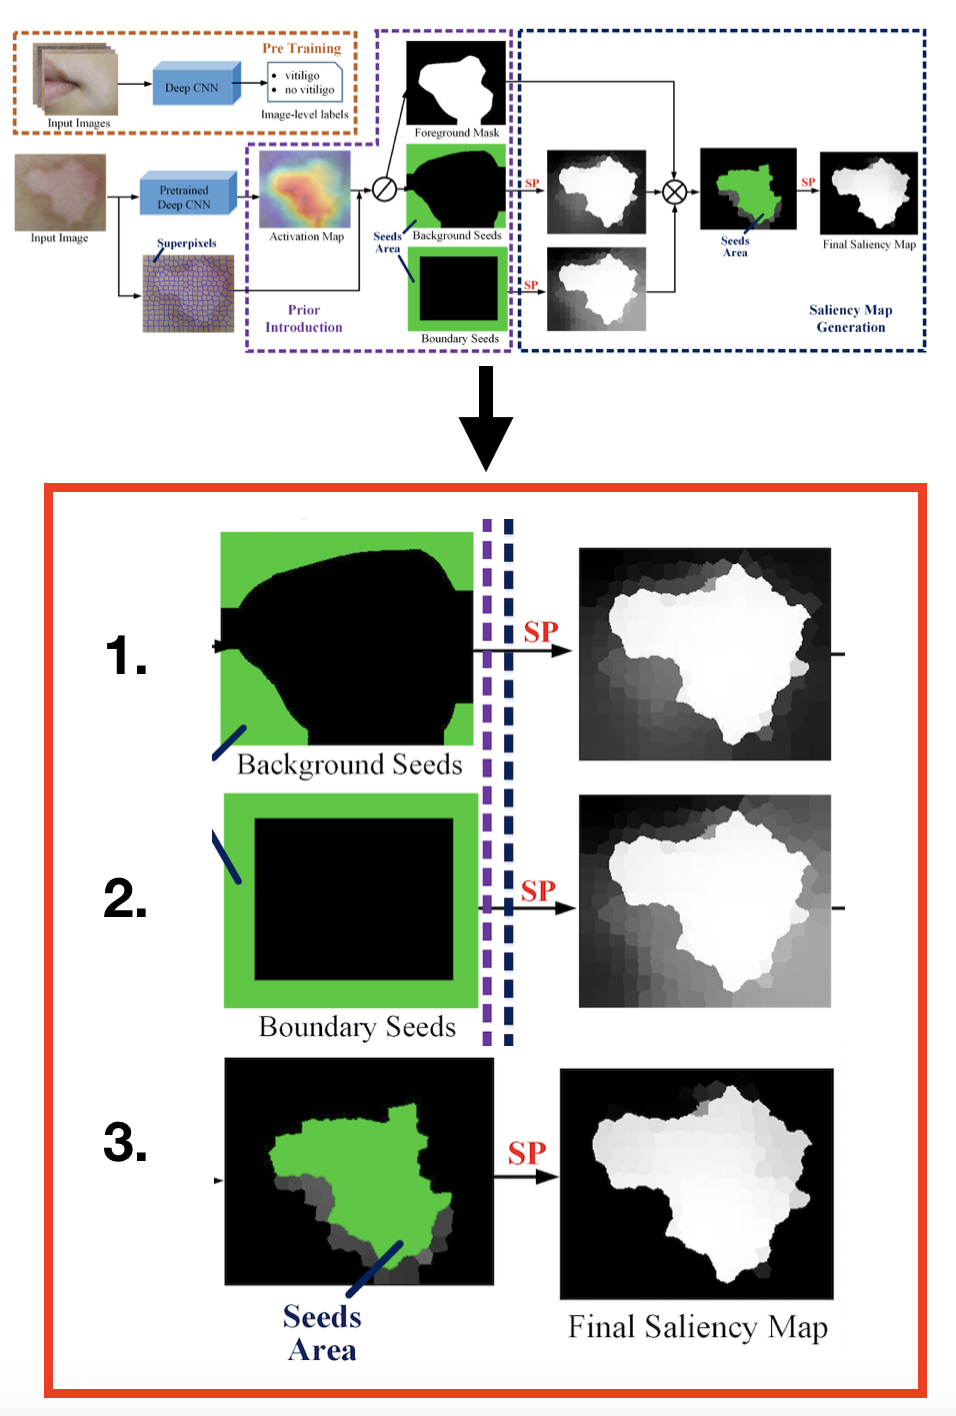
\includegraphics[width=\linewidth]{figures/slaiencyquality.png}
\end{figure}

\column{.6\textwidth}
\begin{figure}
    \centering
    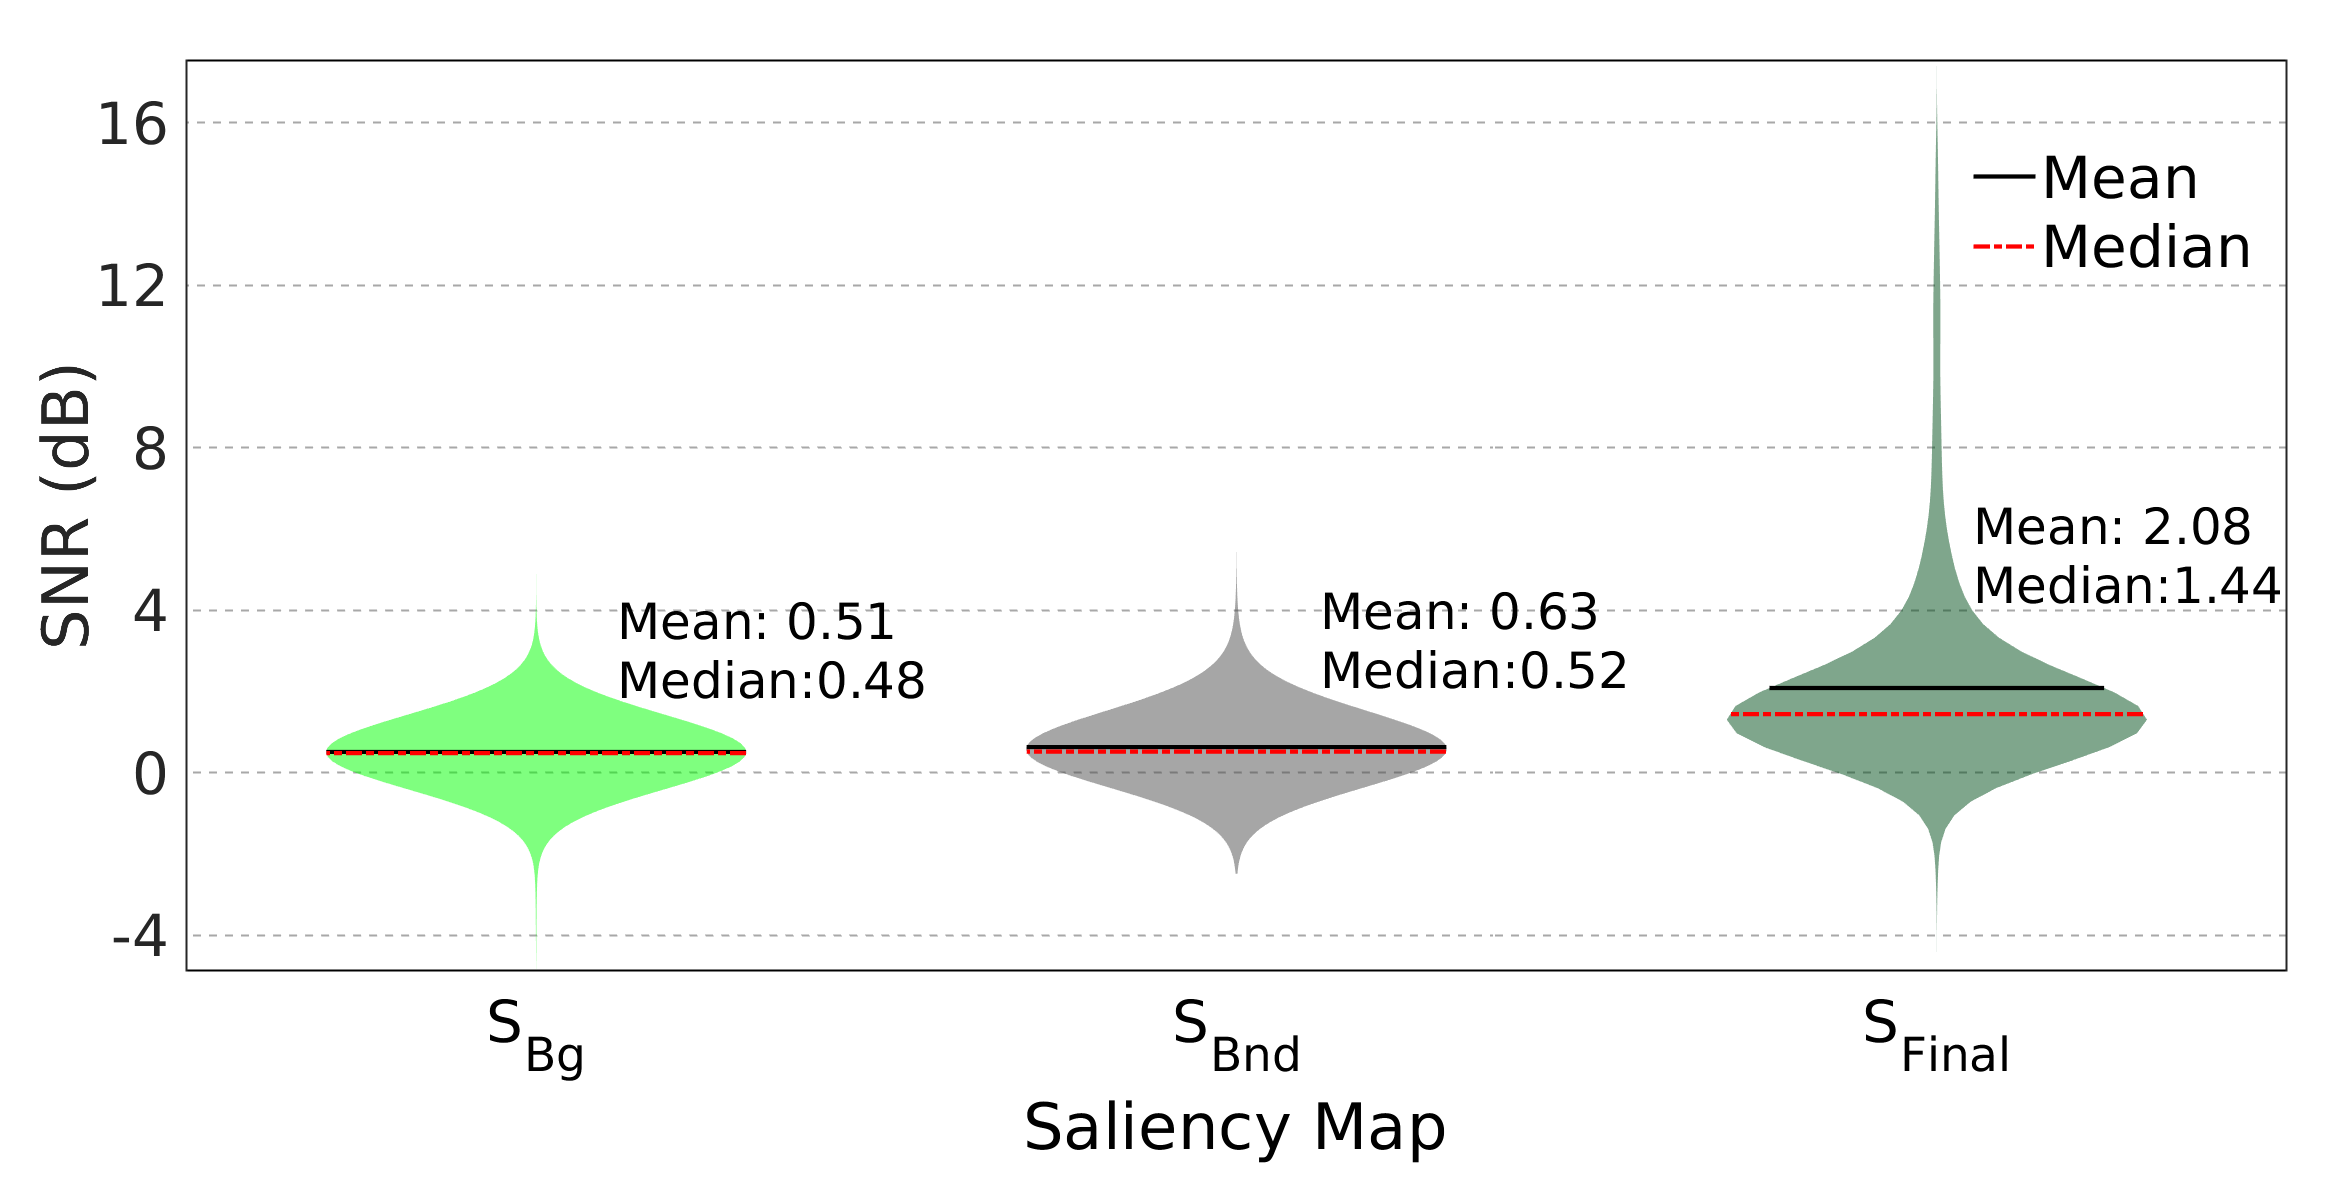
\includegraphics[width=\linewidth]{figures/VitViolin.eps}
\end{figure}

\vspace{-.4cm}

\begin{block}{定义}\small
信号:皮损区域内的显著性值

噪声:皮损区域外的显著性值
\end{block}

\vspace{-.2cm}

\begin{equation}\small
\mathrm{SNR_{dB}}=10\mathrm{log_{10}}(\frac{E_{\mathrm{signal}}}{E_{\mathrm{noise}}}) \nonumber
\end{equation}
\end{columns}
\end{frame}
%%%
\begin{frame}{Ablation Study}
\begin{figure}
    \centering
    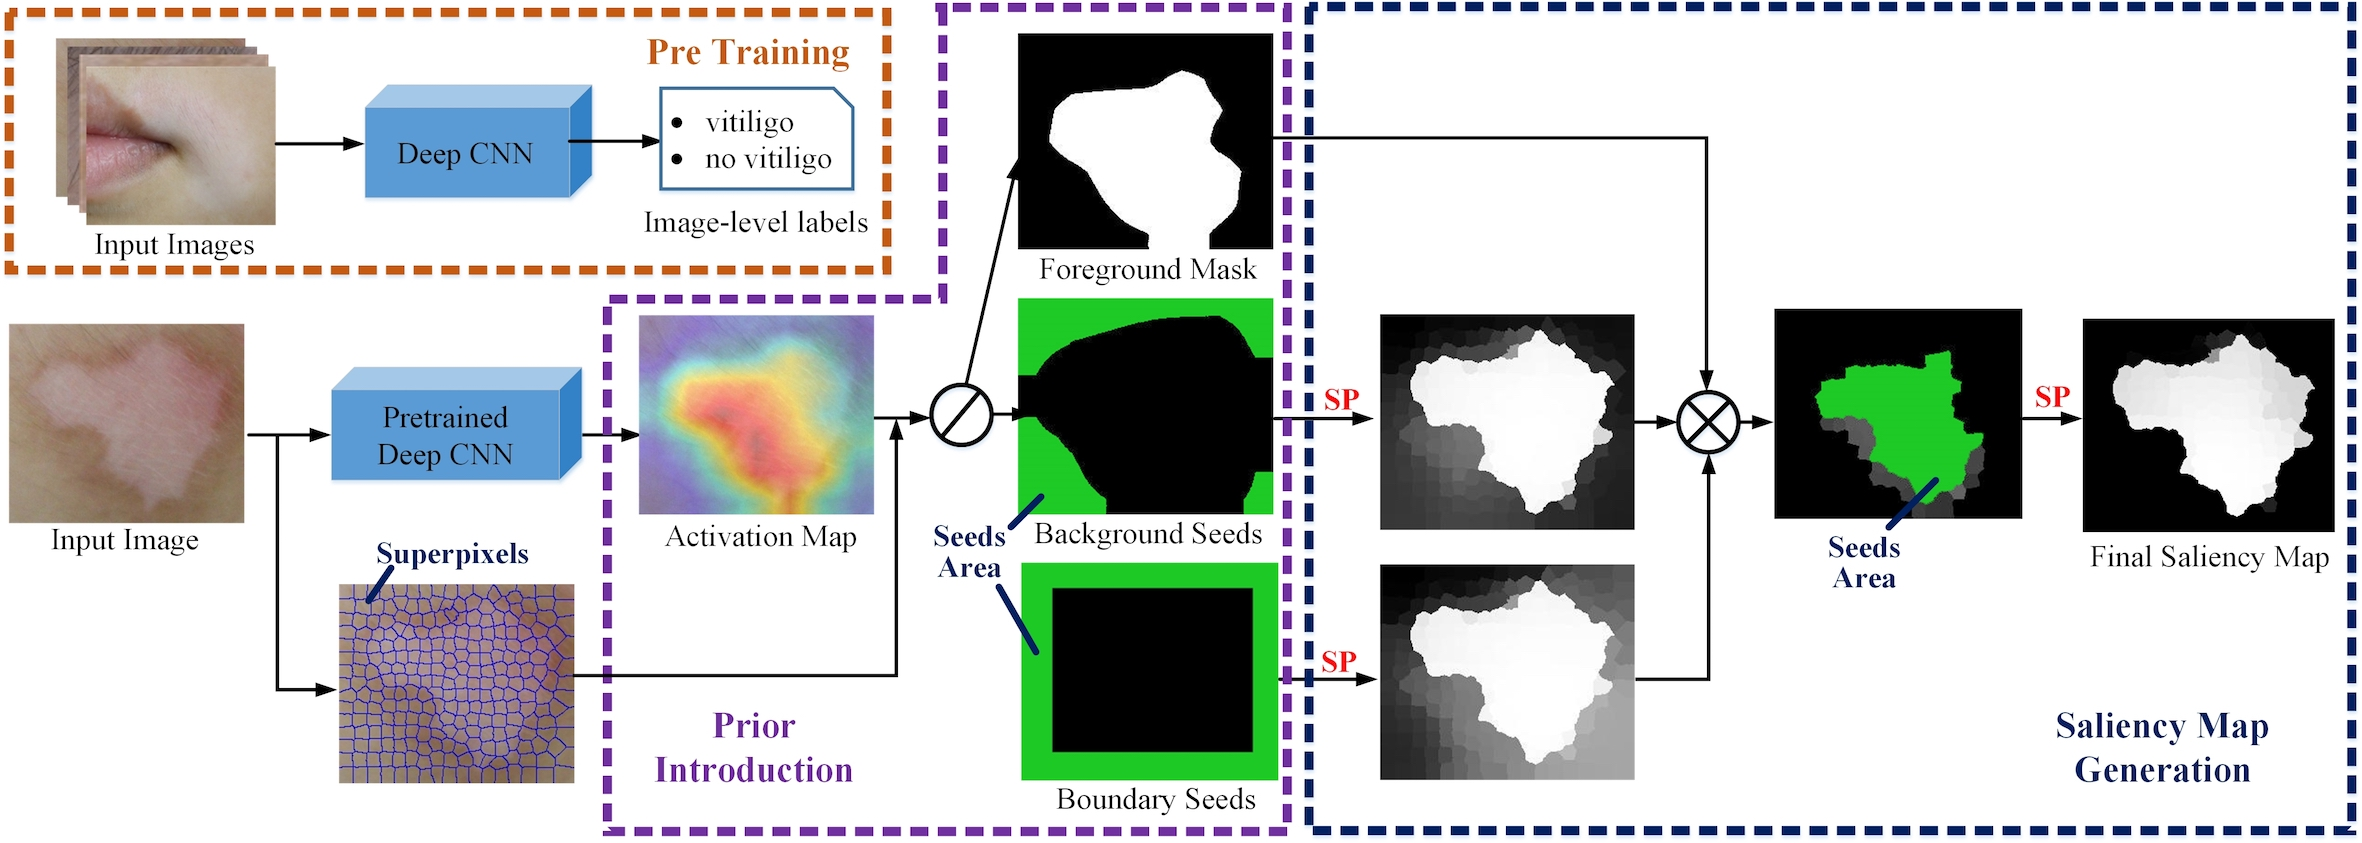
\includegraphics[width=0.9\linewidth]{figures/CNNandSuperPixelModelGraph3.jpg}
\end{figure}
\vfill
\begin{table}[]
\label{tab:ablation}
\begin{center}
\setlength{\tabcolsep}{1 mm}{
    \begin{tabular}{c|cccccccc}
    \toprule
    Fg Mask & \xmark &   \cmark    &    \cmark   &   \cmark    & \xmark & \xmark & \xmark & \cmark \\
    Bg Seeds &  \cmark     & \xmark &   \cmark    & \xmark &  \cmark     & \xmark &  \cmark     & \cmark \\
    Bnd Seeds &  \cmark     &   \cmark    & \xmark & \xmark & \xmark &   \cmark    &   \cmark    & \cmark \\
    Last SP &   \cmark    &   \cmark    & \cmark      &   \cmark    &  \cmark     &    \cmark   &\xmark & \cmark \\
    \midrule
    IoU  & 62.5  & 66.7  & 63.1  & 59.5  & 43.5  & 53.0  & 57.7  & \textbf{71.4}  \\
    \bottomrule
    \end{tabular}}%
\end{center}
\end{table}%
\end{frame}
%%%
\begin{frame}{敏感度测试}
\begin{figure}
    \centering
    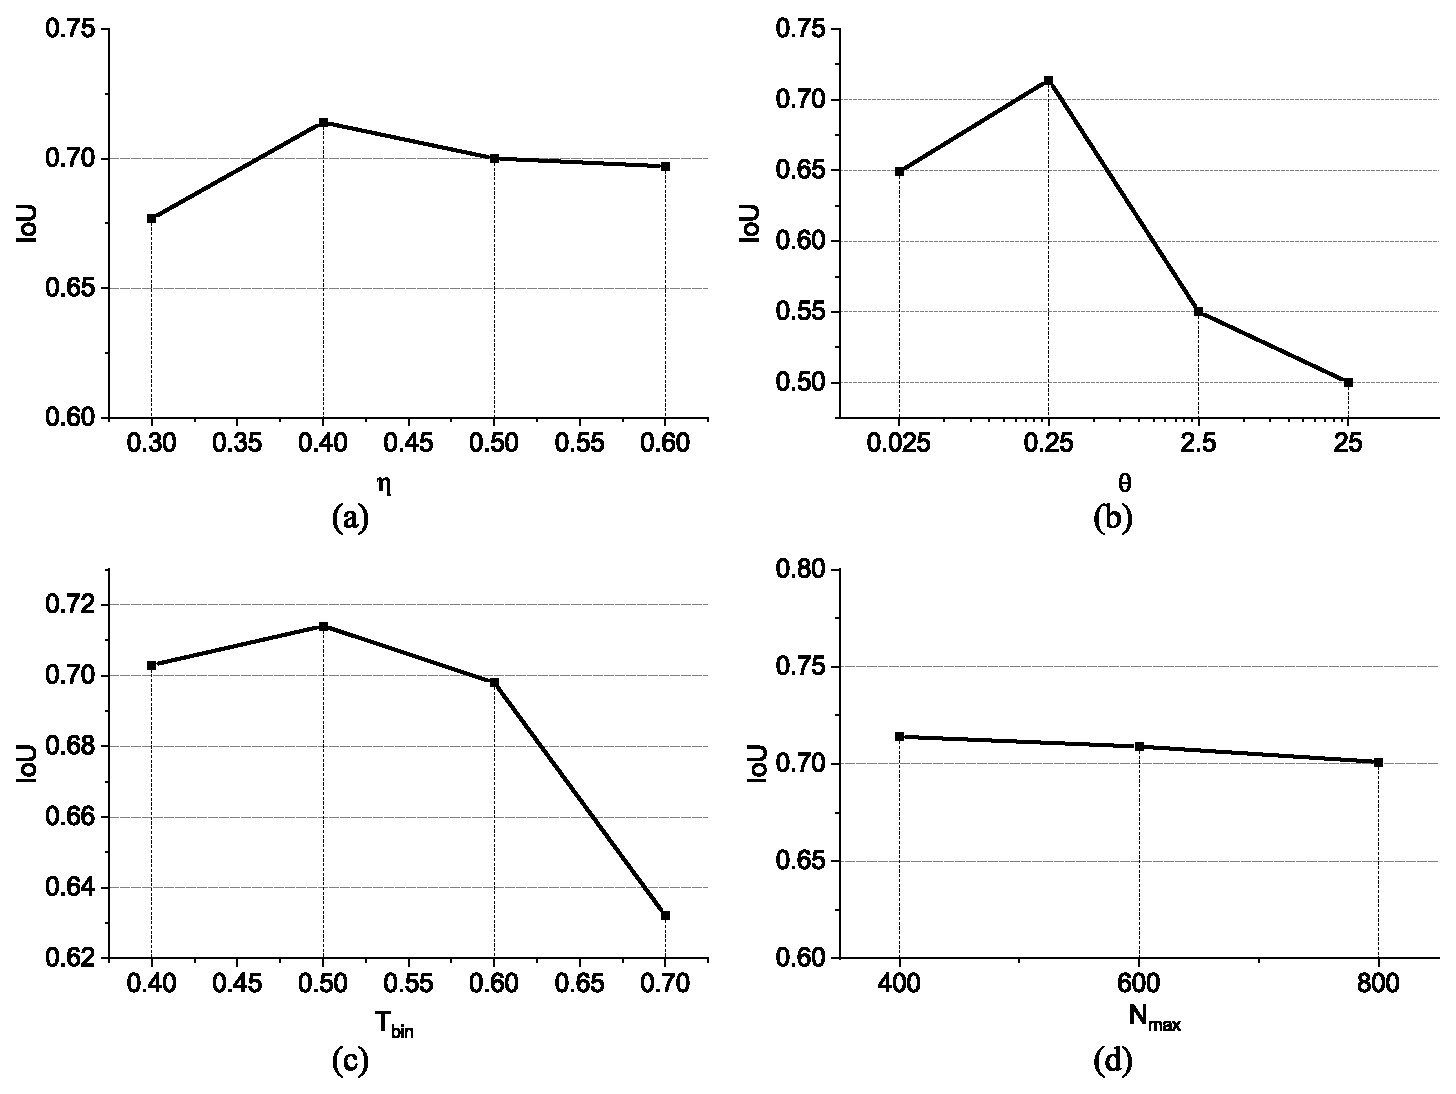
\includegraphics[width=0.8\linewidth]{figures/composit1.eps}
\end{figure}
\end{frame}










\section{讨论与展望}
\begin{frame}{工作总结}
工作量:
\begin{itemize}
\item Vit2019: 目前最大的白癜风分割数据集
\item 大量的实验验证
\item 撰写论文和专利
\end{itemize}

\vspace{0.1cm}

创新点:
\begin{itemize}
\item 基于显著性传播的弱监督分割方法:
\begin{itemize}
\item 应用超像素技术
\item ``既见树木,又见森林''策略
\item 将反馈思想与显著性传播相结合
\end{itemize}
\end{itemize}

\vspace{0.1cm}

其他工作:
\begin{itemize}
\item 集成分割算法到皮研所系统
\end{itemize}

\vspace{-0.2cm}

\begin{figure}
    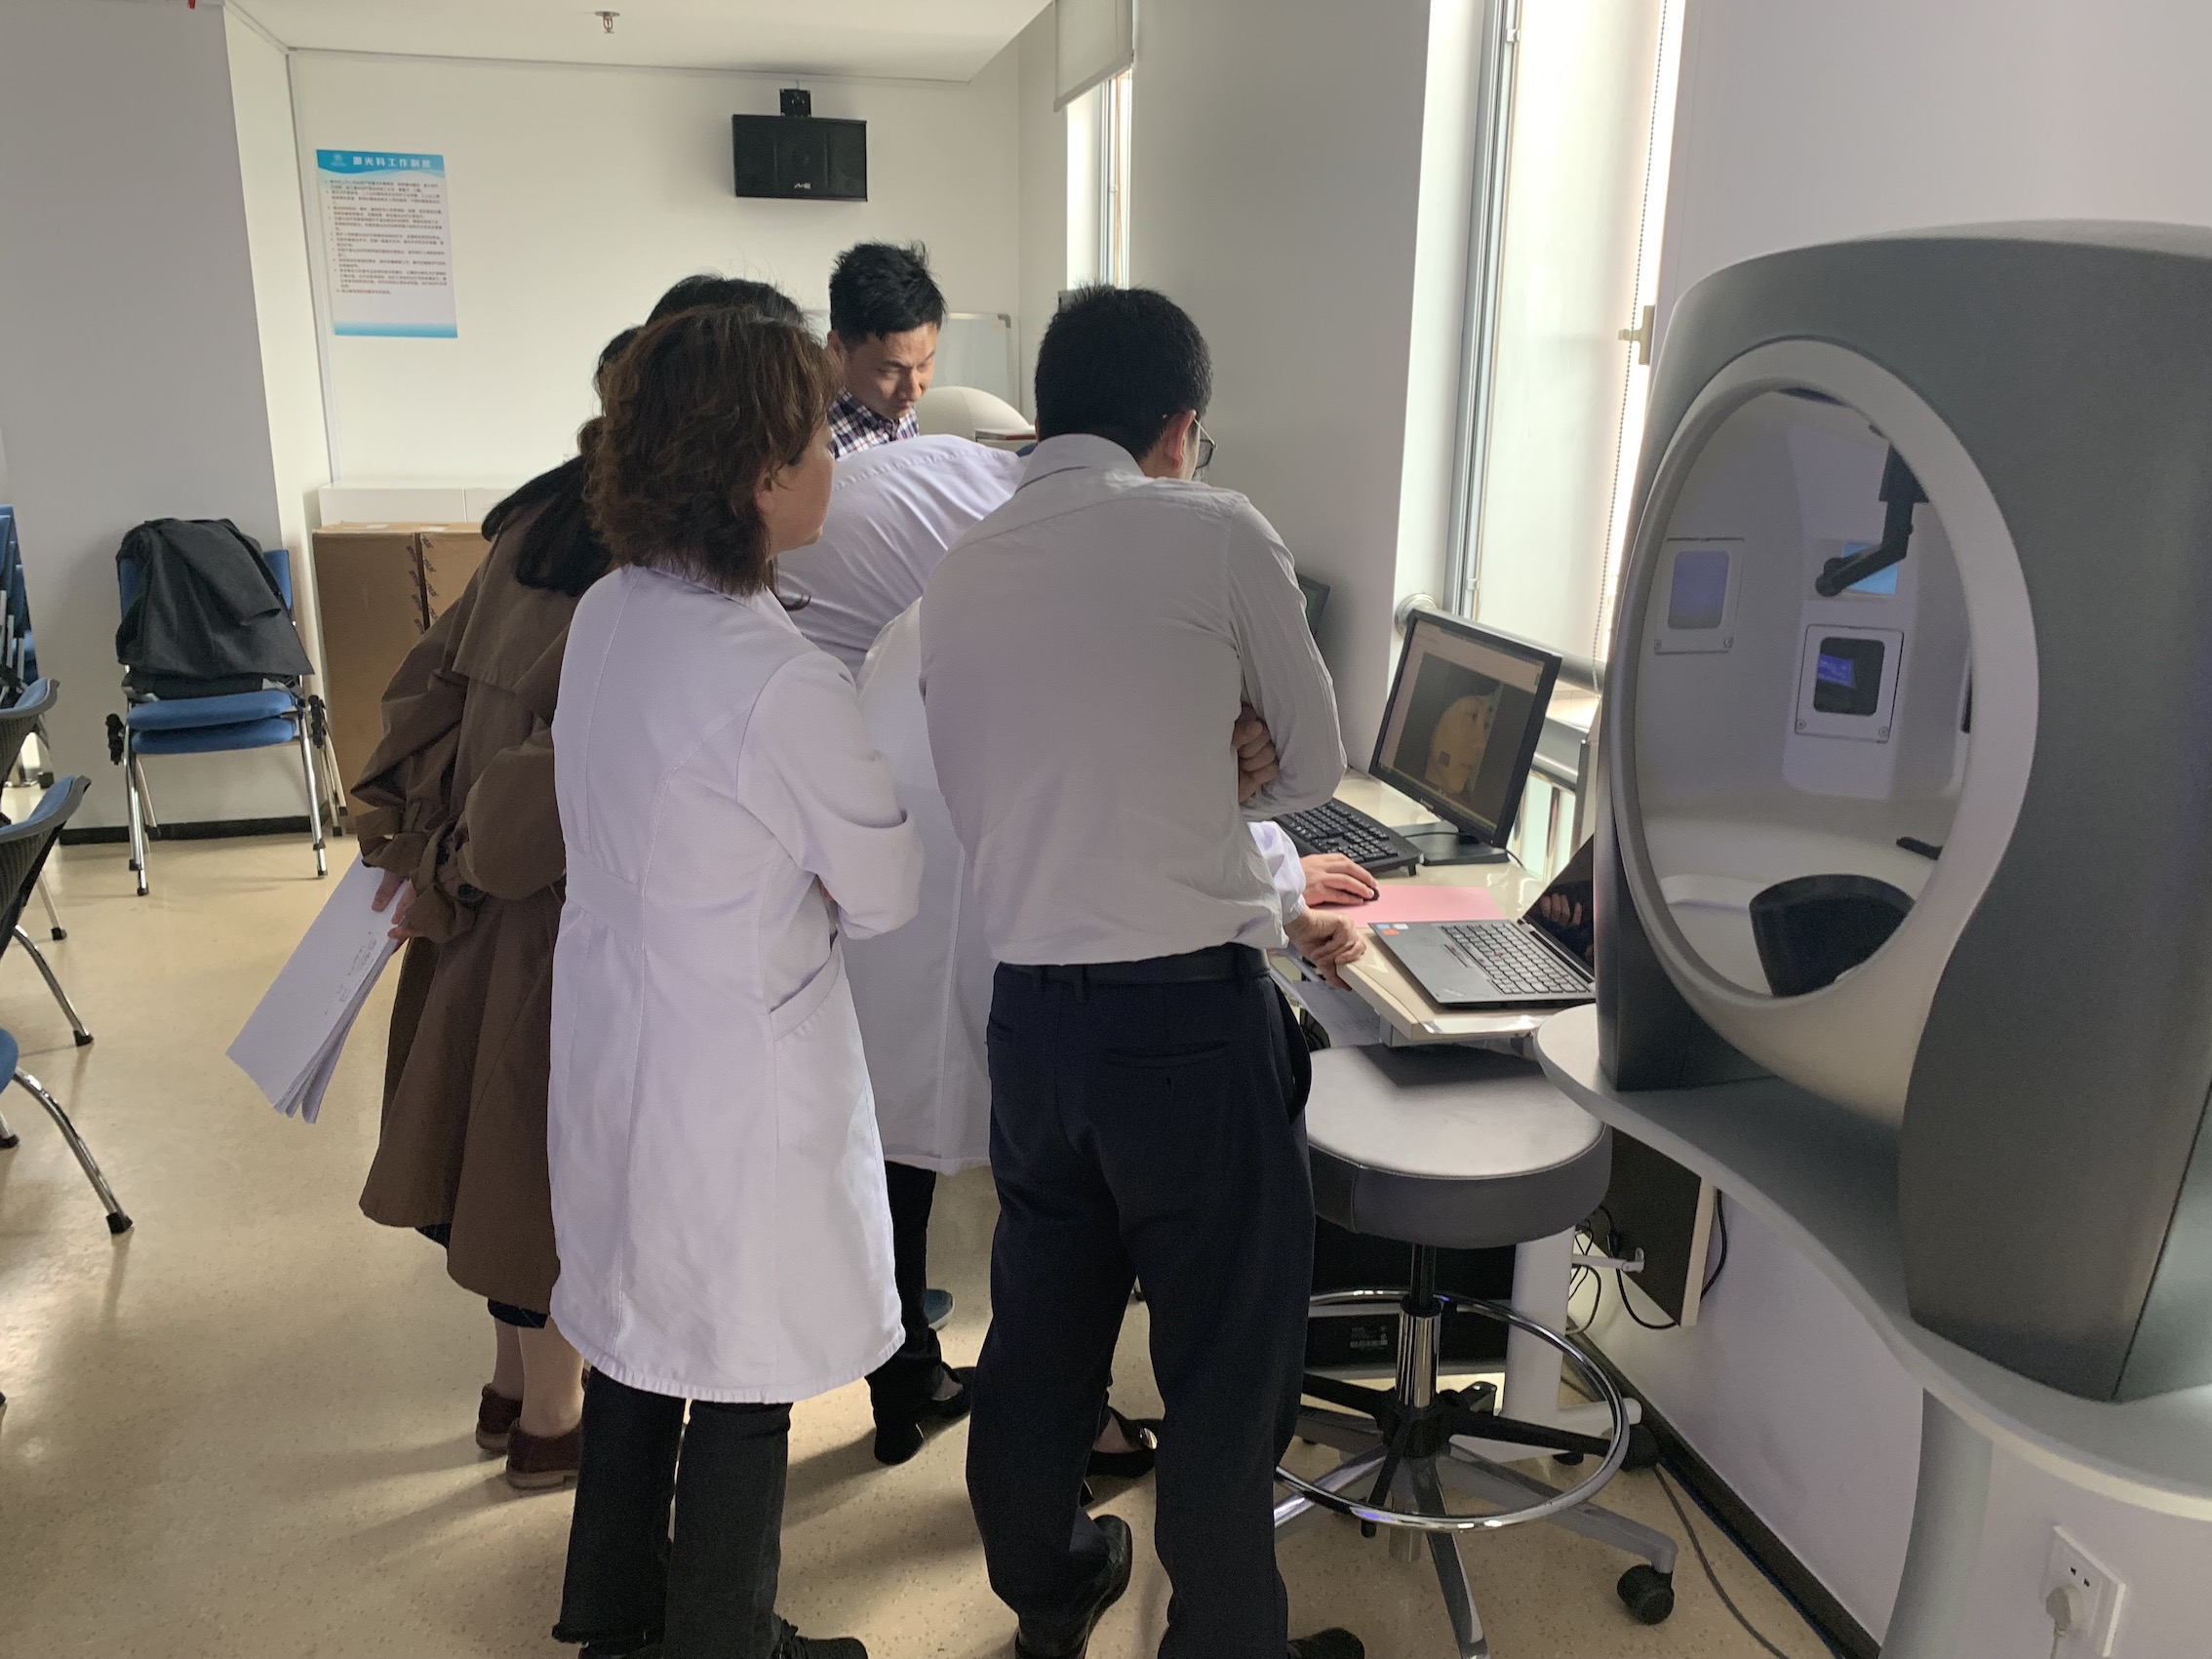
\includegraphics[width=.26\linewidth]{figures/presentation2.jpg}
    \hspace{0.05cm}
    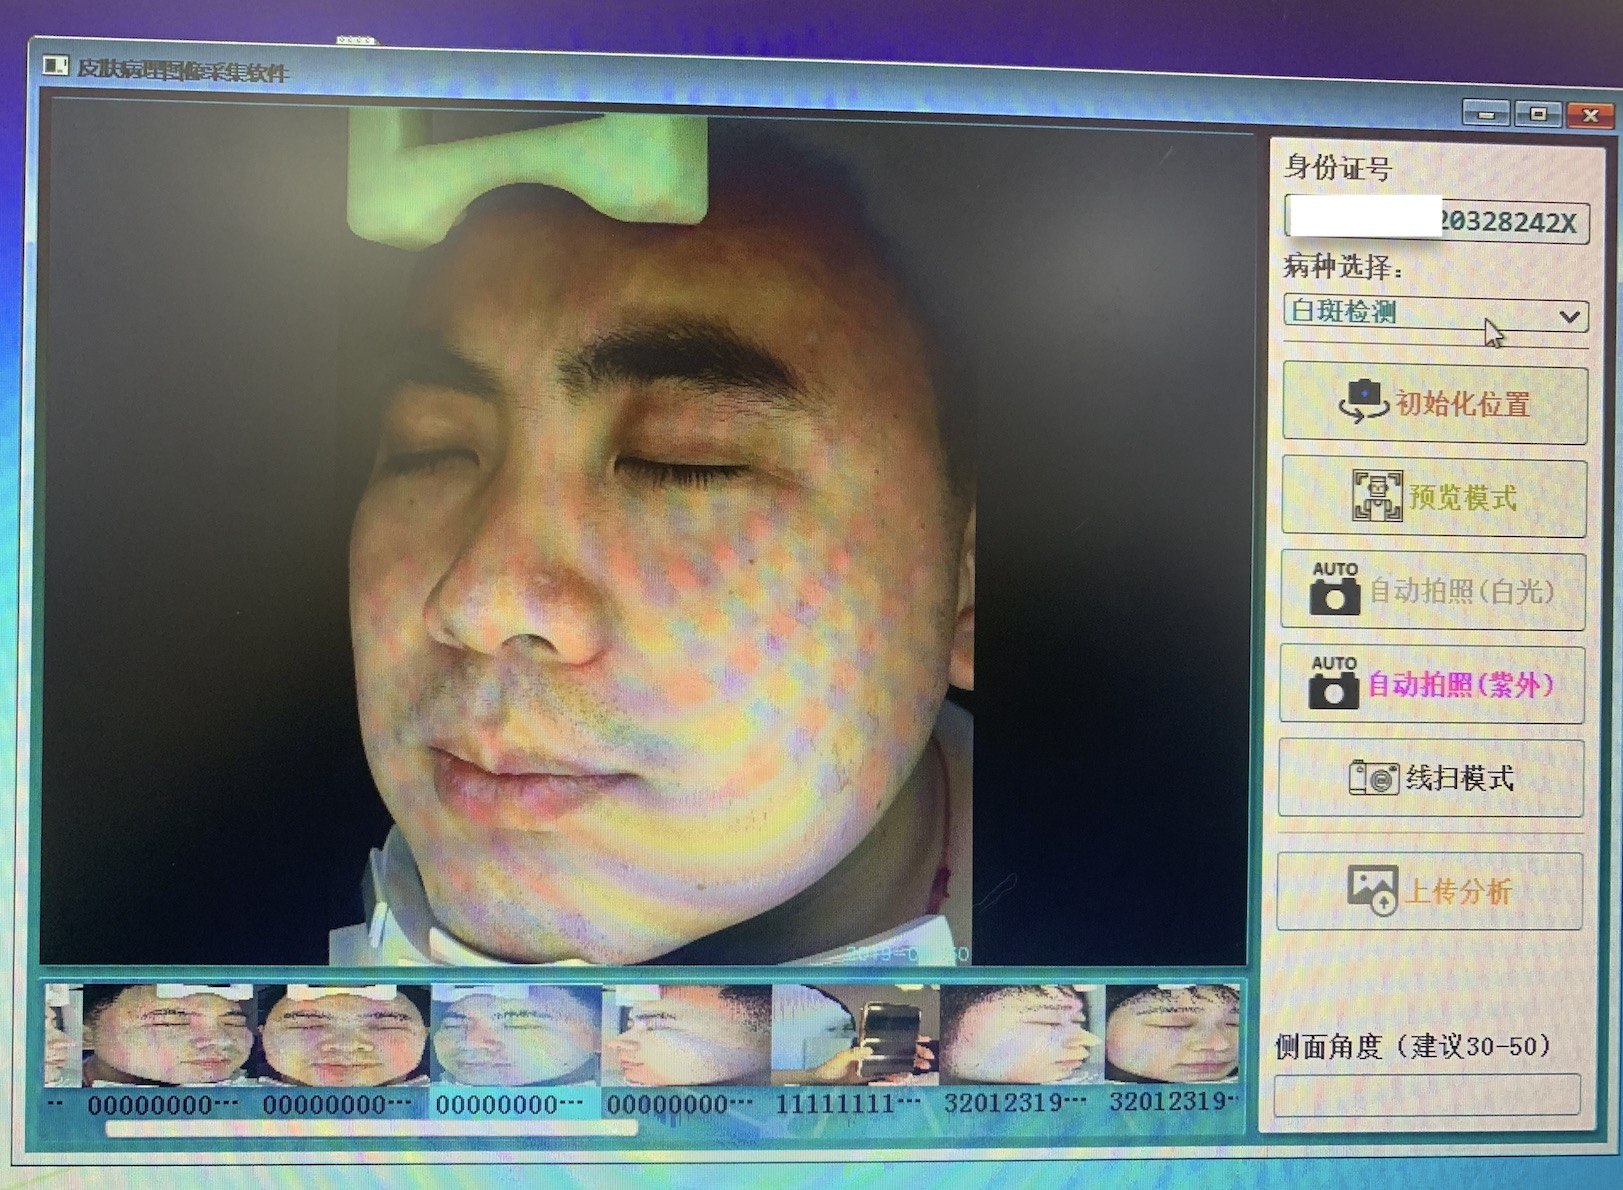
\includegraphics[width=.26\linewidth]{figures/presentation1.jpg}
\end{figure}
\end{frame}
%其他工作:
%\begin{columns}
%\column{.5\textwidth}
%\begin{itemize}
%\item 集成分割算法到皮研所系统
%\end{itemize}
%\column{.5\textwidth}
%\begin{figure}
%    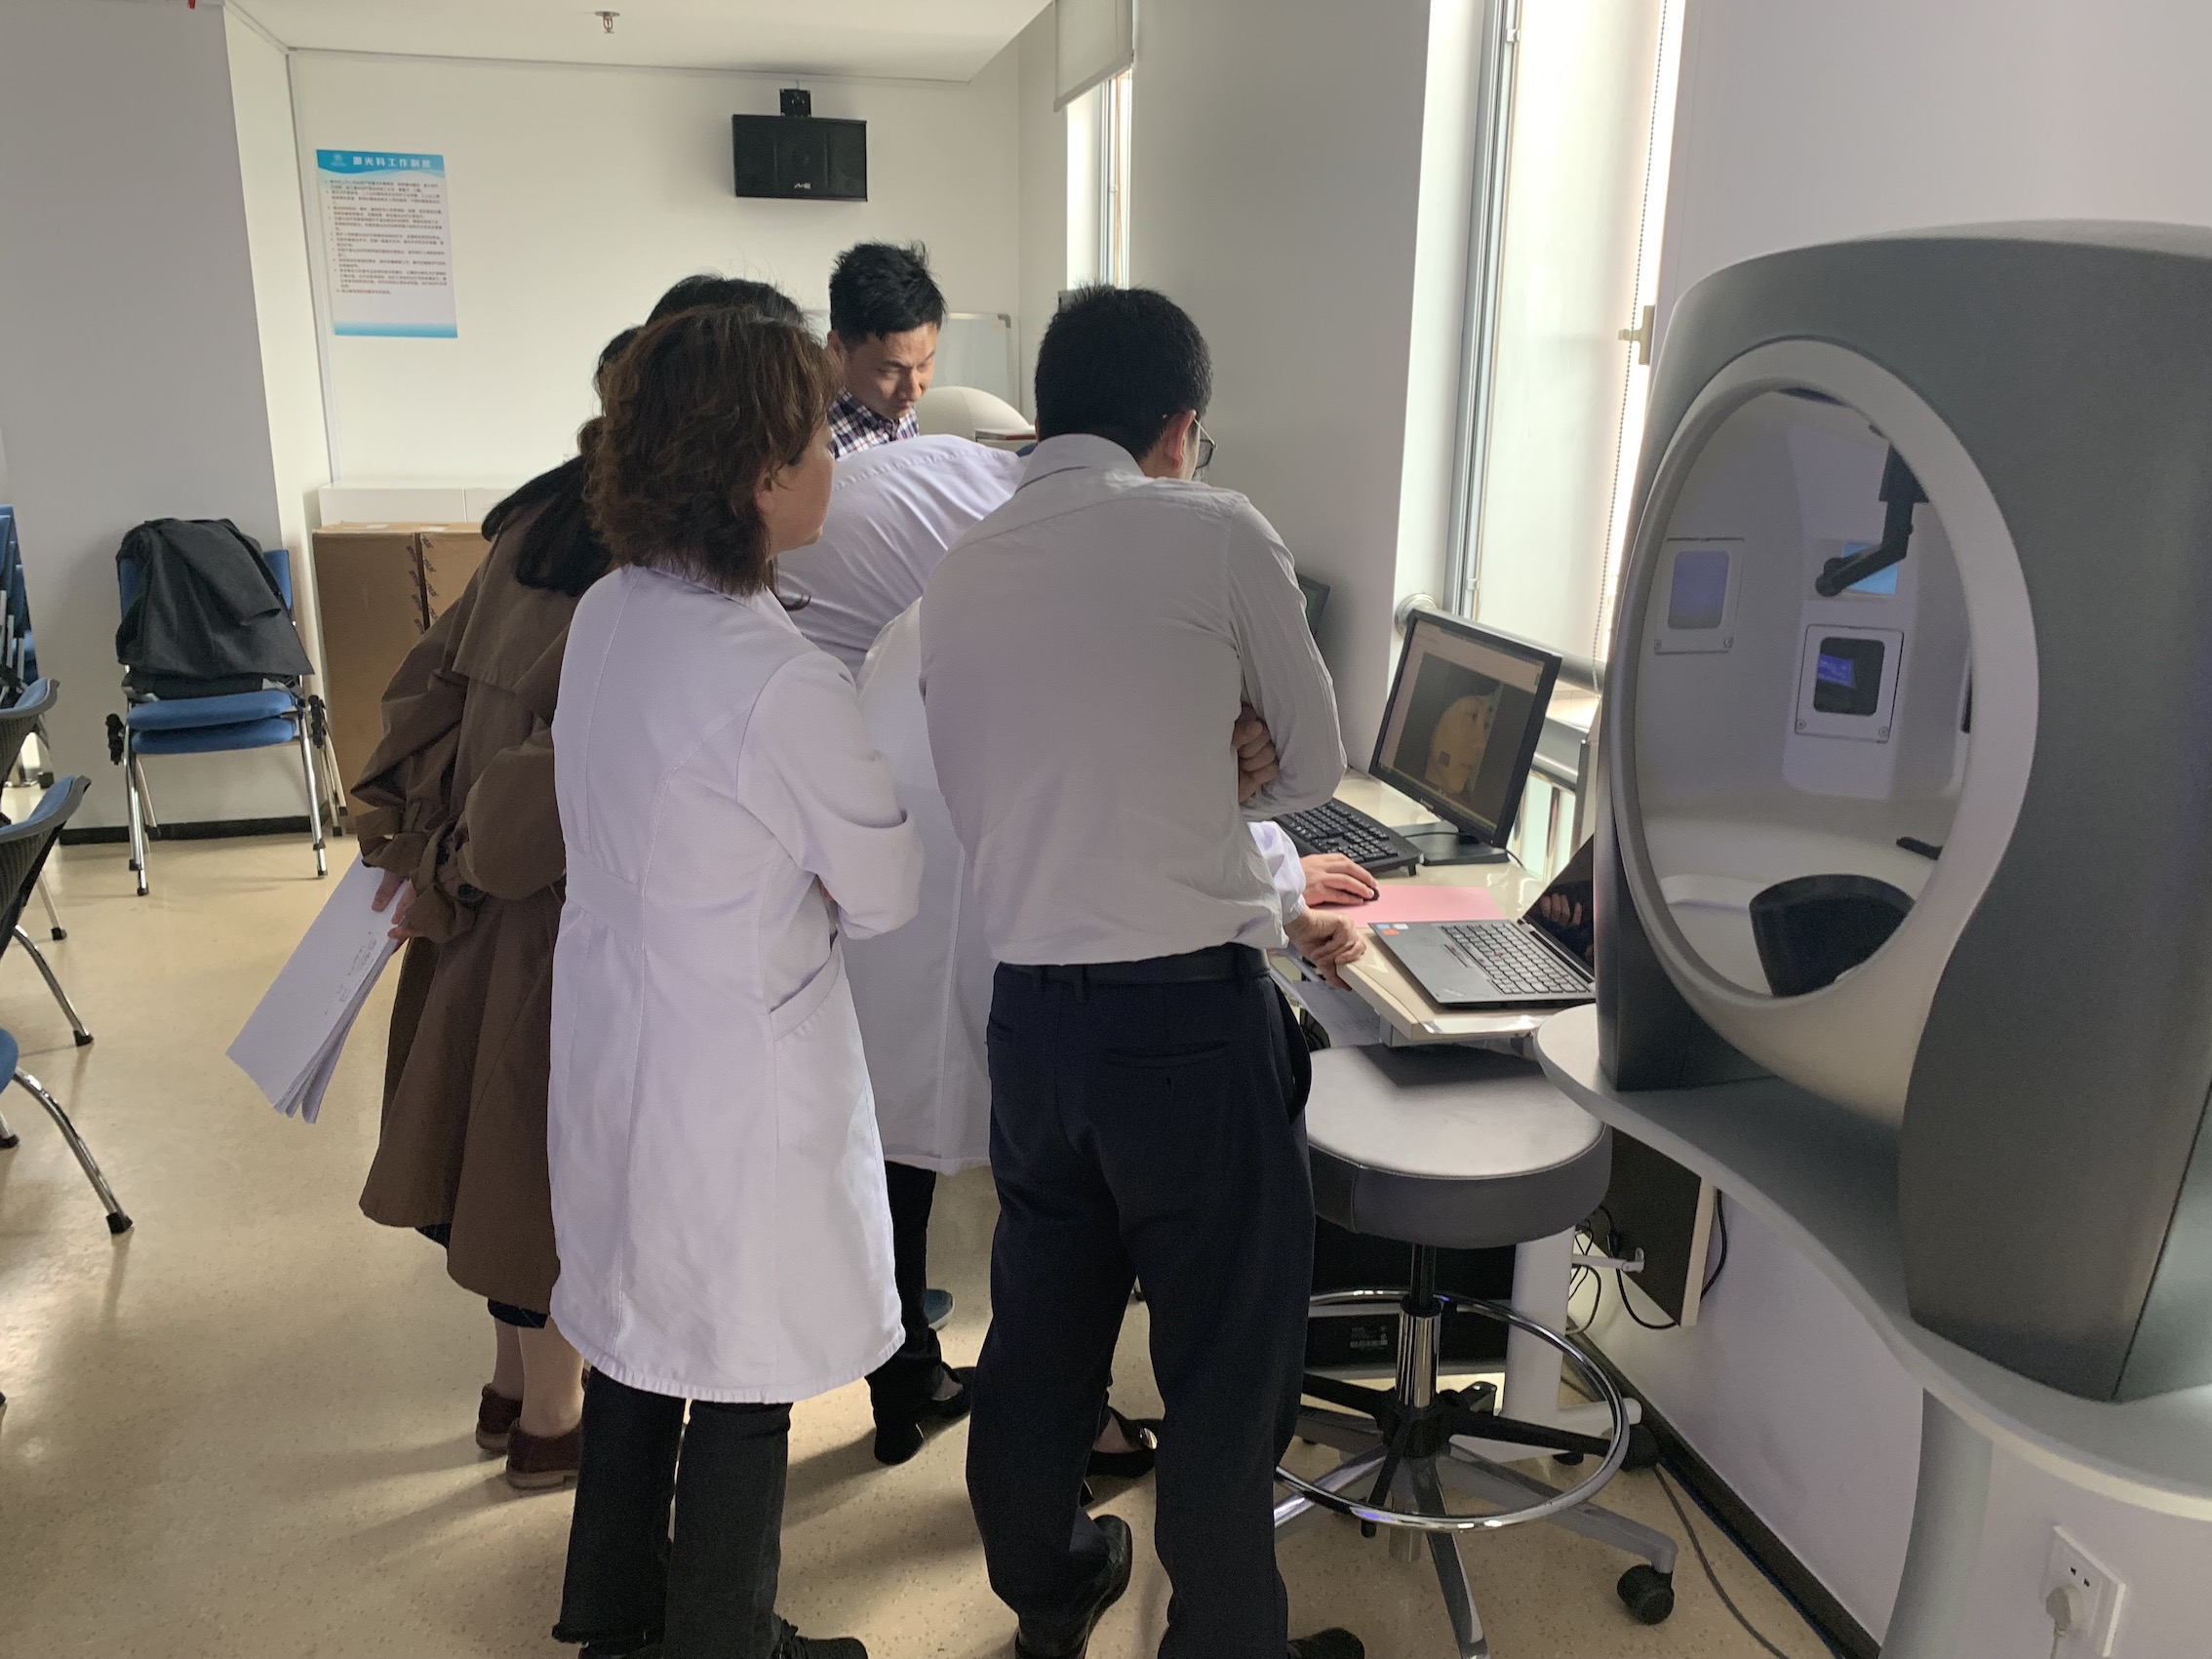
\includegraphics[width=.48\linewidth]{figures/presentation2.jpg}
%    \hspace{0.05cm}
%    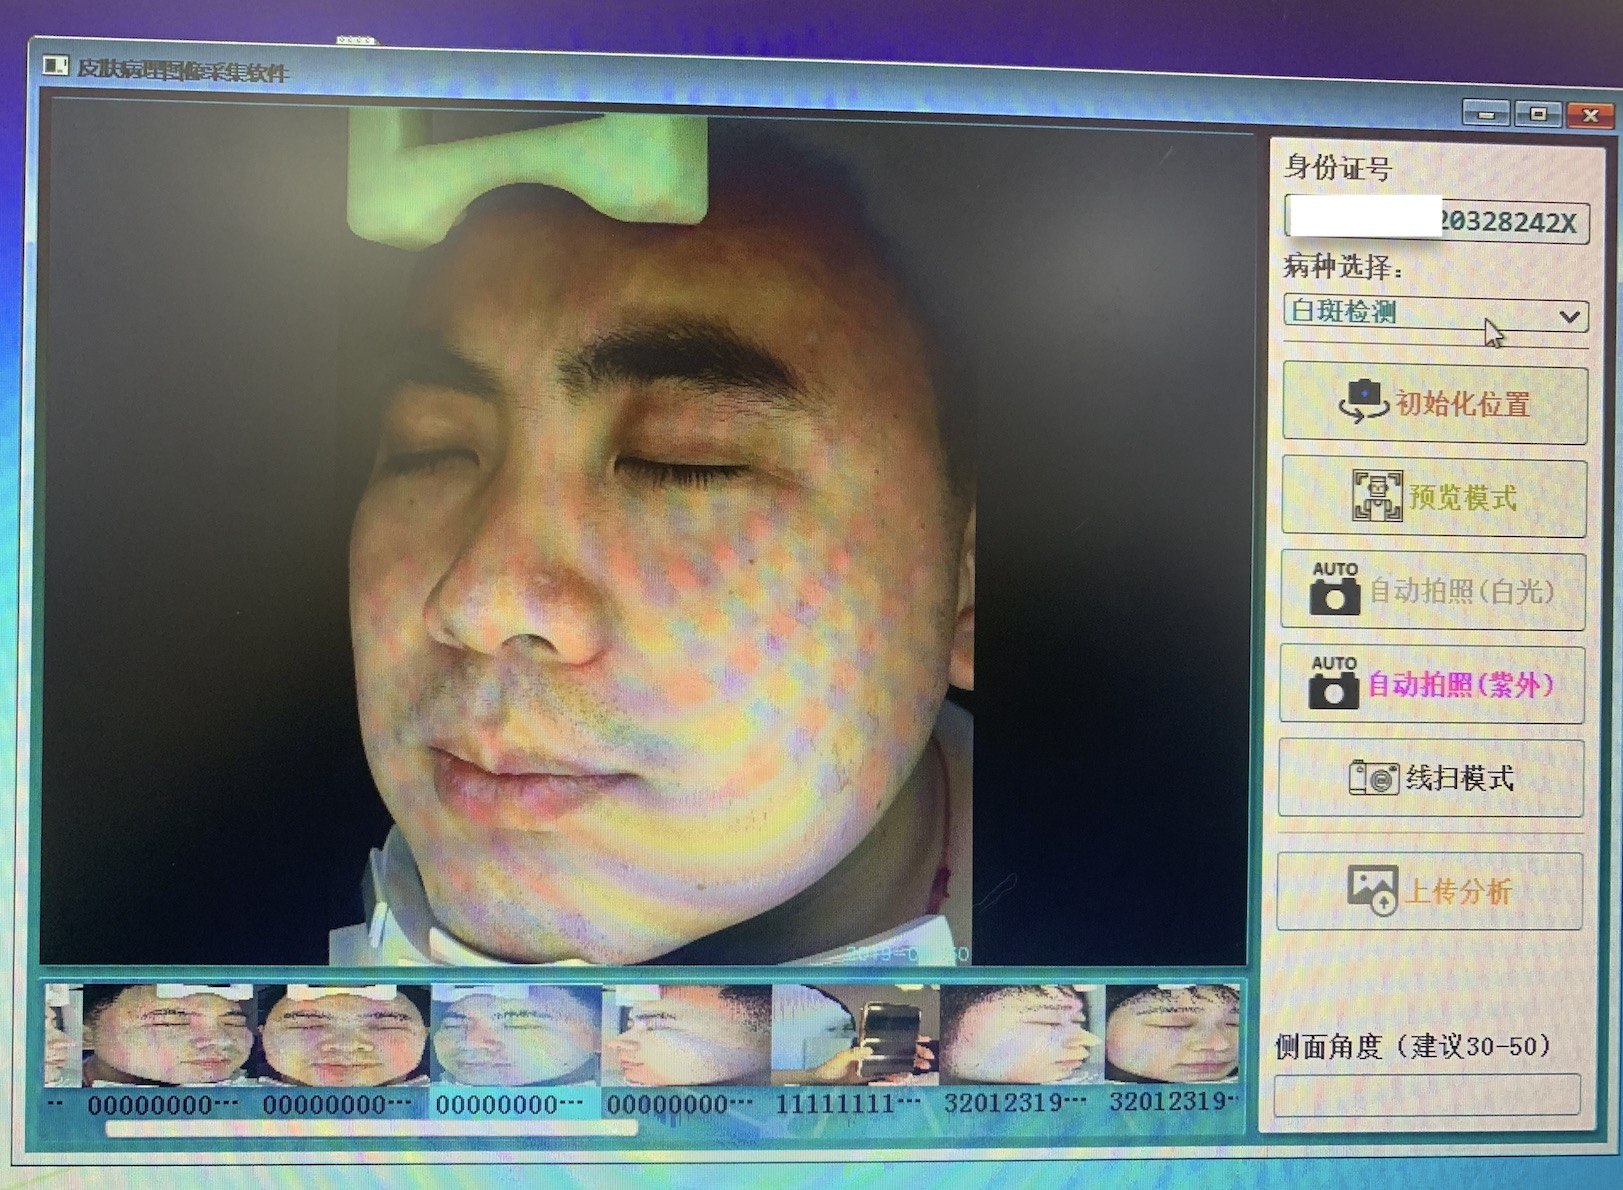
\includegraphics[width=.48\linewidth]{figures/presentation1.jpg}
%\end{figure}
%\end{columns}


%%%
\begin{frame}{工作总结}
论文\footnote{\tiny \textbf{Zhangxing Bian, Siyu Xia}, Chao Xia, Ming Shao, FU YUN. Weakly Supervised Vitiligo
Segmentation in Skin Image through Saliency Propagation.\textit{In Proceedings of the IEEE
international conference on computer vision, 2019}}(于3月投稿ICCV\footnote{\tiny 计算机视觉领域三大顶会之一})
\hspace{2.5cm}专利\footnote{\tiny 发明人:\textbf{边张行, 夏思宇}; 公布号:CN 109741336 A}(已公开)
\begin{figure}
    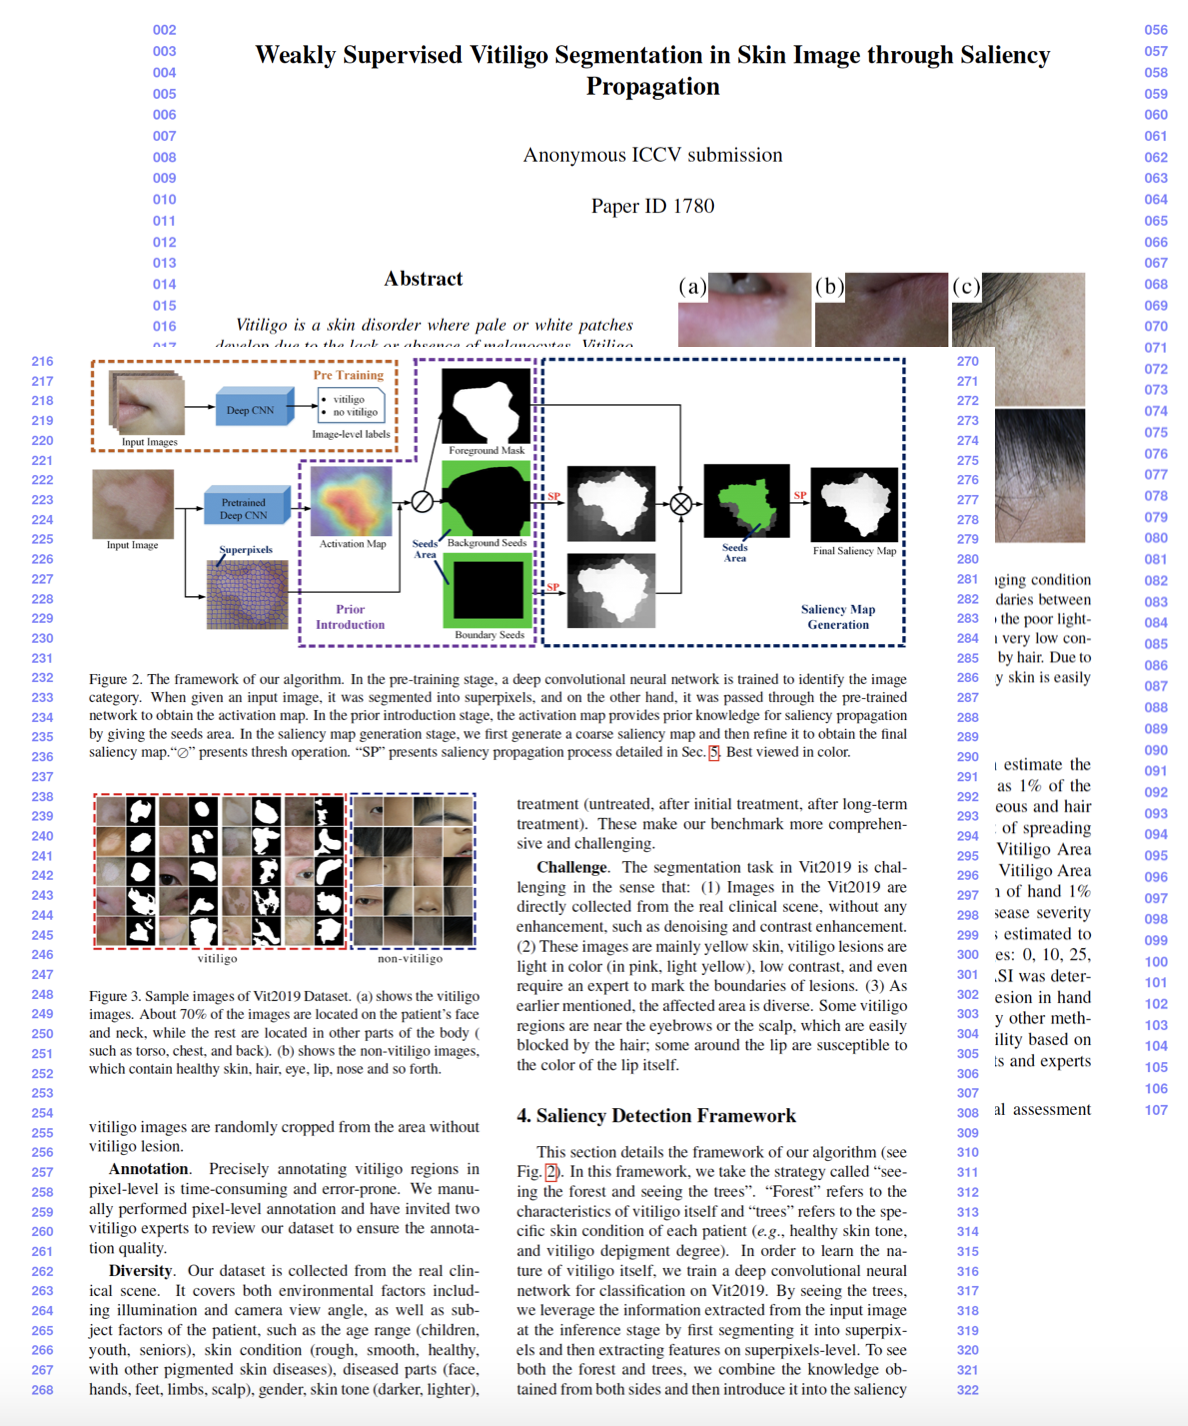
\includegraphics[width=.4\linewidth]{figures/paperFigure.png}
    \hfill
    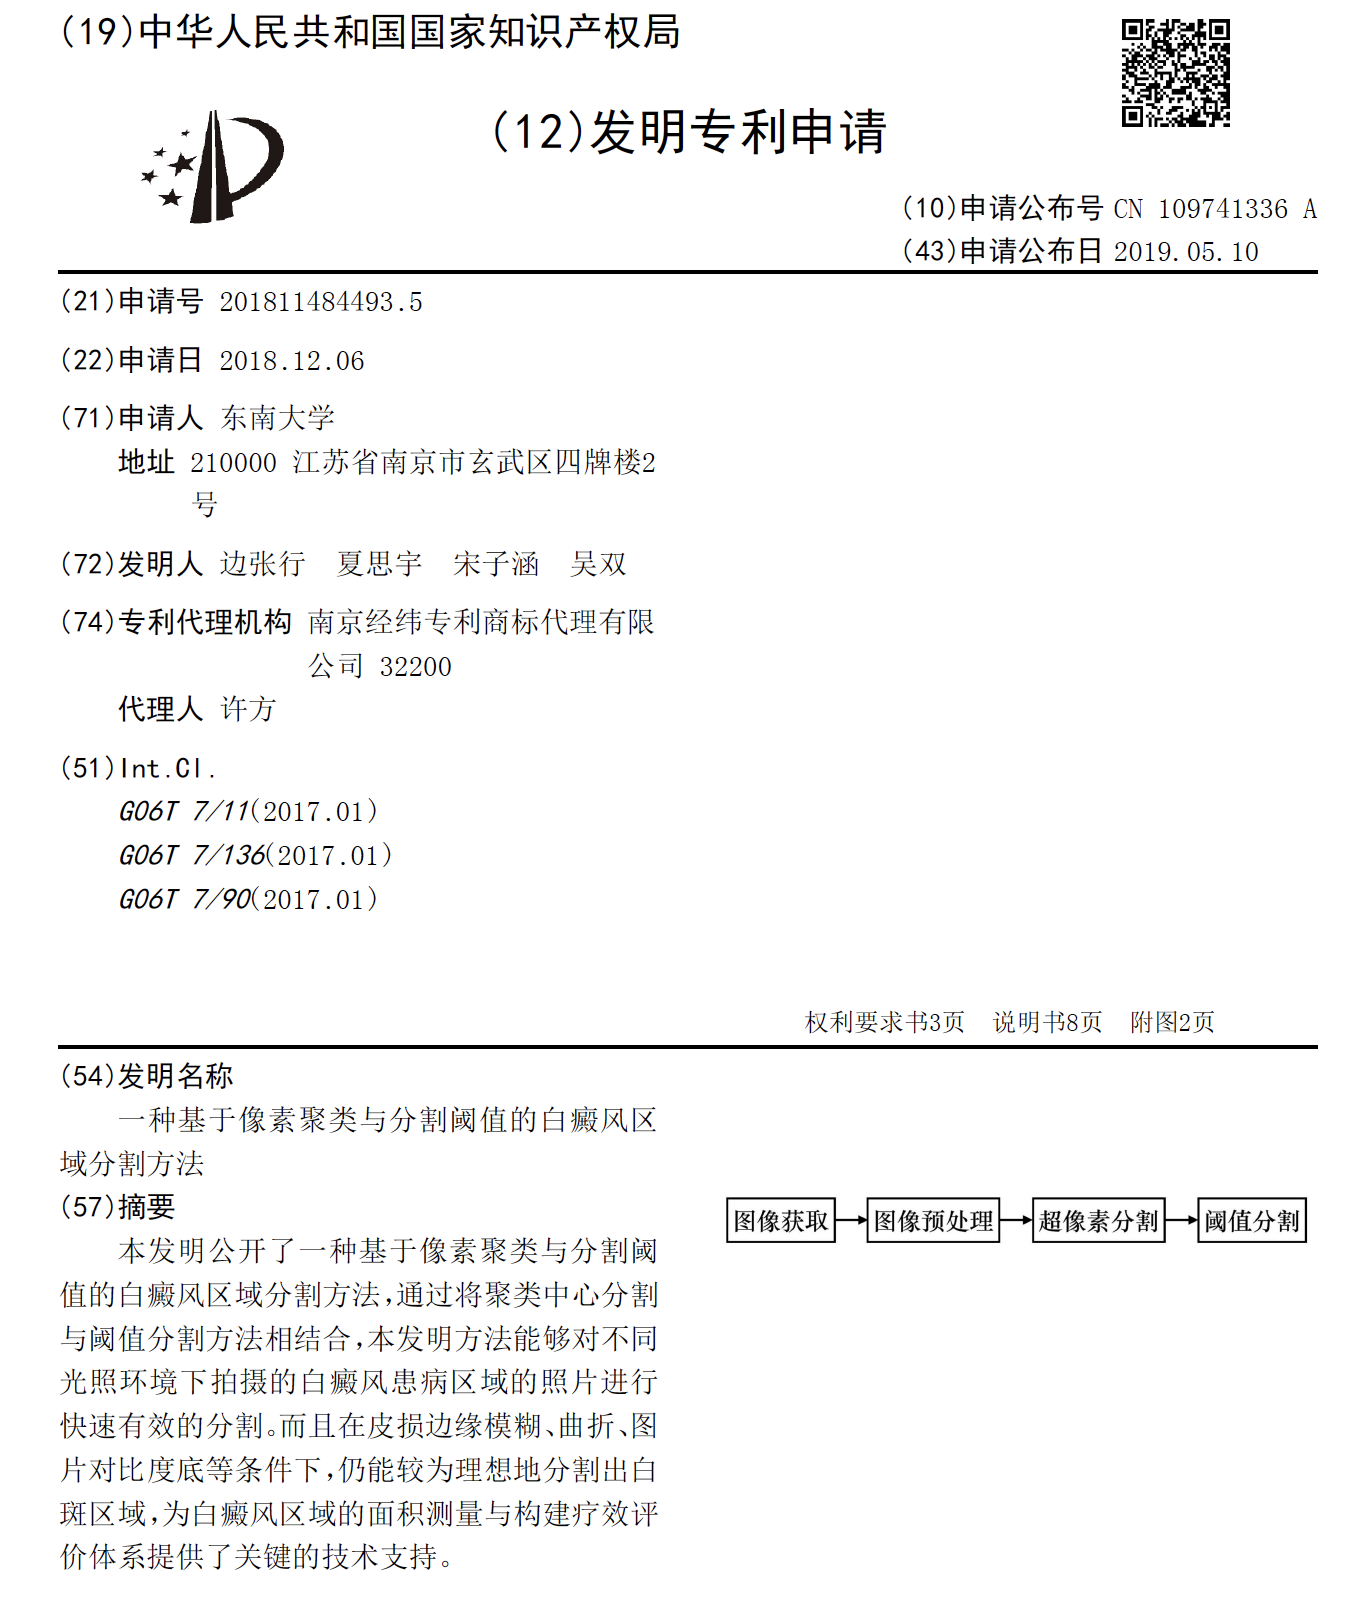
\includegraphics[width=.4\linewidth]{figures/patent.png}
\end{figure}
\end{frame}
%%%
\begin{frame}{展望}
\begin{itemize}
\item 应用:弱监督分割+交互式标注
\item 应用:其他皮损区域的分割 e.g. 黄褐斑、雀斑、烧伤
\begin{figure}
    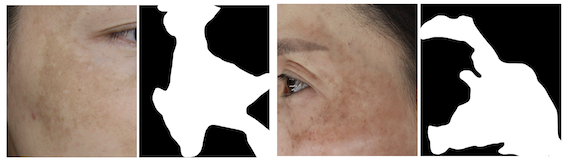
\includegraphics[width=.6\linewidth]{figures/meldemo.png}
\end{figure}

\item 计算皮损区域的绝对物理面积~$\Rightarrow$~3D人脸模型
\end{itemize}

\begin{figure}
    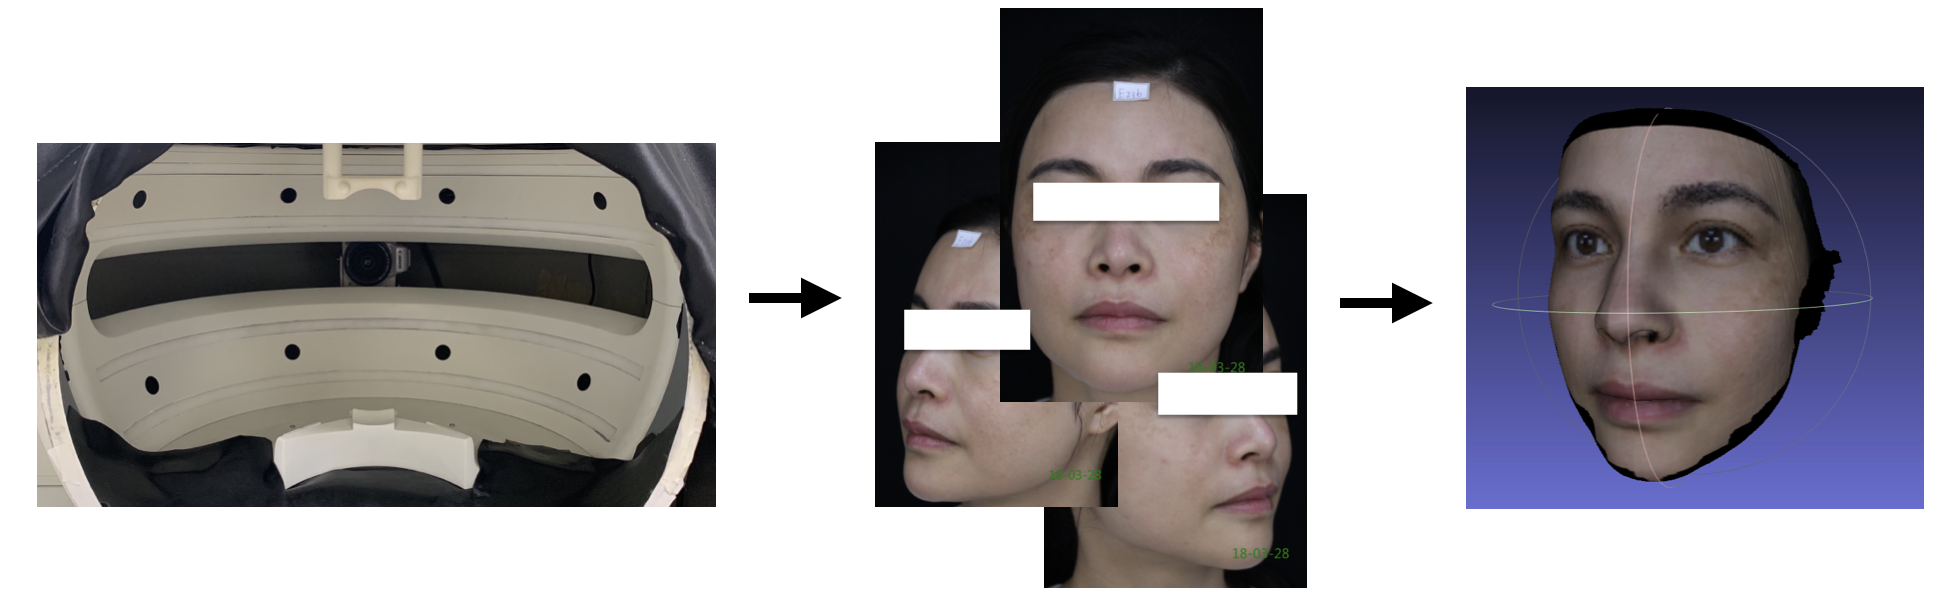
\includegraphics[width=.9\linewidth]{figures/statCamera.png}
\end{figure}

\end{frame}


\begin{frame}{}
\centering \huge
致谢

\vspace{.8cm}

\Large
感谢{\color{blue}{夏思宇}}老师!

\vspace{.4cm}

感谢{\color{blue}{钱堃}}、{\color{blue}{王雁刚}}、{\color{blue}{王辰星}}老师在相关领域给与的启发和帮助!

\vspace{.4cm}

感谢各位评审老师的聆听!
\end{frame}




















%\begin{frame}[allowframebreaks]{References}
%\def\newblock{}
%\nocite{*} % list references without cite them in text
%{\tiny
%\bibliographystyle{ieee}
%\bibliography{References}
%}
%\end{frame}


\end{document}